\documentclass[11pt]{article}

\usepackage[T1]{fontenc}
\usepackage{lmodern}
\usepackage[margin=0.90in]{geometry}
\usepackage{microtype}
\usepackage{amsmath,amssymb,amsthm,mathtools}
\usepackage{booktabs,longtable,array,tabularx}
\usepackage{graphicx}
\usepackage{float}
\usepackage{xcolor}
\usepackage{enumitem}
\usepackage{fancyhdr}
\usepackage{hyperref}
\usepackage[nameinlink,noabbrev]{cleveref}
\usepackage{listings}
\usepackage{caption}
\usepackage{bm}
\usepackage{needspace}
\usepackage{placeins}

\graphicspath{{figures/}}
\allowdisplaybreaks

\hypersetup{
  pdftitle={Projector-Resolved Seed Calculus V},
  pdfauthor={Komorebi P.},
  pdfsubject={Polyphase signal calculus, edge packets, wavelets, and Smith coordinates},
  colorlinks=true,
  linkcolor=black,
  citecolor=black,
  urlcolor=black
}

\pagestyle{fancy}
\fancyhf{}
\fancyhead[L]{Projector-Resolved Seed Calculus V}
\fancyhead[R]{Komorebi P.}
\fancyfoot[C]{\thepage}
\setlength{\headheight}{14pt}

\newtheorem{theorem}{Theorem}[section]
\newtheorem{proposition}[theorem]{Proposition}
\newtheorem{lemma}[theorem]{Lemma}
\newtheorem{corollary}[theorem]{Corollary}
\theoremstyle{definition}
\newtheorem{definition}[theorem]{Definition}
\newtheorem{example}[theorem]{Example}
\newtheorem{construction}[theorem]{Construction}
\newtheorem{conjecture}[theorem]{Conjecture}
\theoremstyle{remark}
\newtheorem{remark}[theorem]{Remark}
\newtheorem{boundary}[theorem]{Boundary}
\newtheorem{certificate}[theorem]{Numerical Certificate}
\newtheorem{classical}[theorem]{Classical Input}

\newcommand{\cA}{\mathcal A}
\newcommand{\cB}{\mathcal B}
\newcommand{\cE}{\mathcal E}
\newcommand{\cF}{\mathcal F}
\newcommand{\cH}{\mathcal H}
\newcommand{\cP}{\mathcal P}
\newcommand{\cR}{\mathcal R}
\newcommand{\cS}{\mathcal S}
\newcommand{\cT}{\mathcal T}
\newcommand{\bbC}{\mathbb C}
\newcommand{\bbR}{\mathbb R}
\newcommand{\bbZ}{\mathbb Z}
\newcommand{\bbN}{\mathbb N}
\newcommand{\Gam}{\Gamma}
\newcommand{\ii}{\mathrm i}
\newcommand{\RMSE}{\operatorname{RMSE}}
\newcommand{\supp}{\operatorname{supp}}
\newcommand{\diag}{\operatorname{diag}}
\newcommand{\lcm}{\operatorname{lcm}}
\newcommand{\IoU}{\operatorname{IoU}}
\newcommand{\rank}{\operatorname{rank}}
\newcolumntype{L}[1]{>{\raggedright\arraybackslash}p{#1}}
\newcolumntype{Y}{>{\raggedright\arraybackslash}X}

\lstset{
  language=Python,
  basicstyle=\ttfamily\footnotesize,
  breaklines=true,
  frame=single,
  showstringspaces=false,
  columns=fullflexible,
  keepspaces=true,
  numbers=left,
  numberstyle=\tiny,
  numbersep=7pt
}

\title{\textbf{Projector-Resolved Seed Calculus V}\\[0.45em]
\large Polyphase Signal Calculus: Exact Reconstruction, Edge Packets, Wavelets, and Smith Coordinates}
\author{Komorebi P.}
\date{}

\begin{document}
\maketitle

\begin{abstract}
This paper develops the signal realization of the projector-resolved seed calculus. The impulse $\delta_0$ is taken as a primitive signal seed and its shift orbit supplies the address system. Residue projectors split a sequence into exact polyphase channels, nested divisibility gives exact refinement, and every finite impulse-response operator becomes a matrix of packet transfers. The standard perfect-reconstruction condition for a filter bank is therefore an analysis--synthesis identity in the common operator language of the series. Haar analysis, wavelet packets, and a predict--update lifting step are treated as explicit finite models. The edge problem is separated into two statements. When a discontinuity packet is known and retained exactly, approximation error is exactly the approximation error of the remaining smooth packet; no spectral approximation of the jump is performed. When the packet is estimated, a symmetric-difference bound isolates mask error, amplitude error, and smooth-background error. Numerical studies compare global Fourier truncation, exact known-packet reconstruction, and a deliberately narrow positive-contrast estimator in one and two dimensions, including curved boundaries, corners, and multiple amplitudes. The same cyclic phase action is then placed on the Smith reflection disk. Its pullback through the Cayley transform is a M\"obius action on impedance, and the two-phase case is precisely impedance--admittance inversion. Nonlinear coefficient products obey cyclic packet convolution. Eighteen code-generated figures, machine-readable results, and thirty-three automated tests accompany the paper. Exact signal theorems, limited numerical estimators, classical constructions, and open recovery problems are kept distinct throughout.
\end{abstract}

\begin{center}
\fbox{\begin{minipage}{0.93\textwidth}
\textbf{Scope and claim boundary.} The paper proves exact polyphase reconstruction, exact finite filter-transfer identities, perfect reconstruction for the stated filter banks, the conditional known-edge theorem, mask and amplitude perturbation bounds, nonlinear residue-convolution laws, and the Smith-coordinate phase action. It does not claim that every discontinuity can be detected automatically, that every form of Gibbs ringing has been eliminated, or that the simple two-class estimator supplied with the release is a universal segmentation method. The estimator is included as one reproducible finite example.  For every finite packet refinement tree, the paper now proves existence of a globally optimal complete pruning, an exact dynamic-programming selector for additive costs, and a deterministic margin-stability certificate. Wavelets, filter banks, the Cayley transform, and the classical Smith grid are treated as classical inputs organized in the common seed--packet--refinement language.
\end{minipage}}
\end{center}

\tableofcontents
\listoffigures
\listoftables
\clearpage

\section{The signal realization of the seed calculus}

Let $\ell^2(\bbZ)$ be the Hilbert space of square-summable discrete signals. Write $\delta_n$ for the unit impulse at address $n$ and let the bilateral shift be
\[
(Sx)[n]=x[n-1].
\]
Then
\[
S^n\delta_0=\delta_n.
\]
The primitive signal seed is therefore $s=\delta_0$, the address operators are the shift words $S^n$, and the completion is the $\ell^2$ norm.

\begin{theorem}[Impulse seed theorem]
The closed shift-generated hull of $\delta_0$ is all of $\ell^2(\bbZ)$:
\[
\boxed{
\overline{\operatorname{span}\{S^n\delta_0:n\in\bbZ\}}^{\,\ell^2}
=\ell^2(\bbZ).
}
\]
Every finitely supported signal has the exact finite expression
\[
x=\sum_{n\in\bbZ}x[n]S^n\delta_0.
\]
\end{theorem}

\begin{proof}
The shift orbit is the standard orthonormal basis $\{\delta_n\}_{n\in\bbZ}$. Finite linear combinations give the finitely supported sequences, which are dense in $\ell^2(\bbZ)$.
\end{proof}

This realization fixes the language used below:
\[
\begin{gathered}
\text{impulse seed}\longrightarrow\text{shift address}\longrightarrow\text{packet projection}\longrightarrow\text{filter transfer}\\
\longrightarrow\text{refinement}\longrightarrow\text{reconstruction}.
\end{gathered}
\]

\begin{remark}[Several completions]
The same algebraic seed description applies to finite sequences, $\ell^1$, $\ell^2$, periodic sequences, tempered distributions, and multidimensional lattices. The topology decides which infinite reconstructions are legitimate. Finite-dimensional experiments in this paper use ordinary Euclidean norms; theorem statements specify the ambient norm when it matters.
\end{remark}

\section{Residue projectors and exact polyphase coordinates}

Fix an integer $N\ge1$. For $0\le r<N$, define
\[
(P_{N,r}x)[n]
=
\mathbf 1_{n\equiv r\, (\mathrm{mod}\,N)}x[n].
\]
The corresponding decimated channel is
\[
x_r[q]=x[Nq+r].
\]

\begin{theorem}[Polyphase projector theorem]
The operators $P_{N,r}$ satisfy
\[
P_{N,r}P_{N,s}=\delta_{rs}P_{N,r},
\qquad
\sum_{r=0}^{N-1}P_{N,r}=I.
\]
Consequently,
\[
\boxed{x=\sum_{r=0}^{N-1}P_{N,r}x}
\]
with no approximation.
\end{theorem}

\begin{proof}
Each integer belongs to exactly one residue class modulo $N$. Multiplying the two indicator functions gives zero for distinct classes and the same indicator for equal classes. Summing all residue indicators gives one at every address.
\end{proof}

Define the analysis and synthesis maps
\[
\cA_Nx=(x_0,\ldots,x_{N-1}),
\qquad
\cS_N(x_0,\ldots,x_{N-1})[Nq+r]=x_r[q].
\]

\begin{corollary}[Analysis--synthesis identity]
\[
\boxed{\cS_N\cA_N=I.}
\]
On the product of the channel spaces one also has $\cA_N\cS_N=I$.
\end{corollary}

\begin{figure}[htbp]
\centering
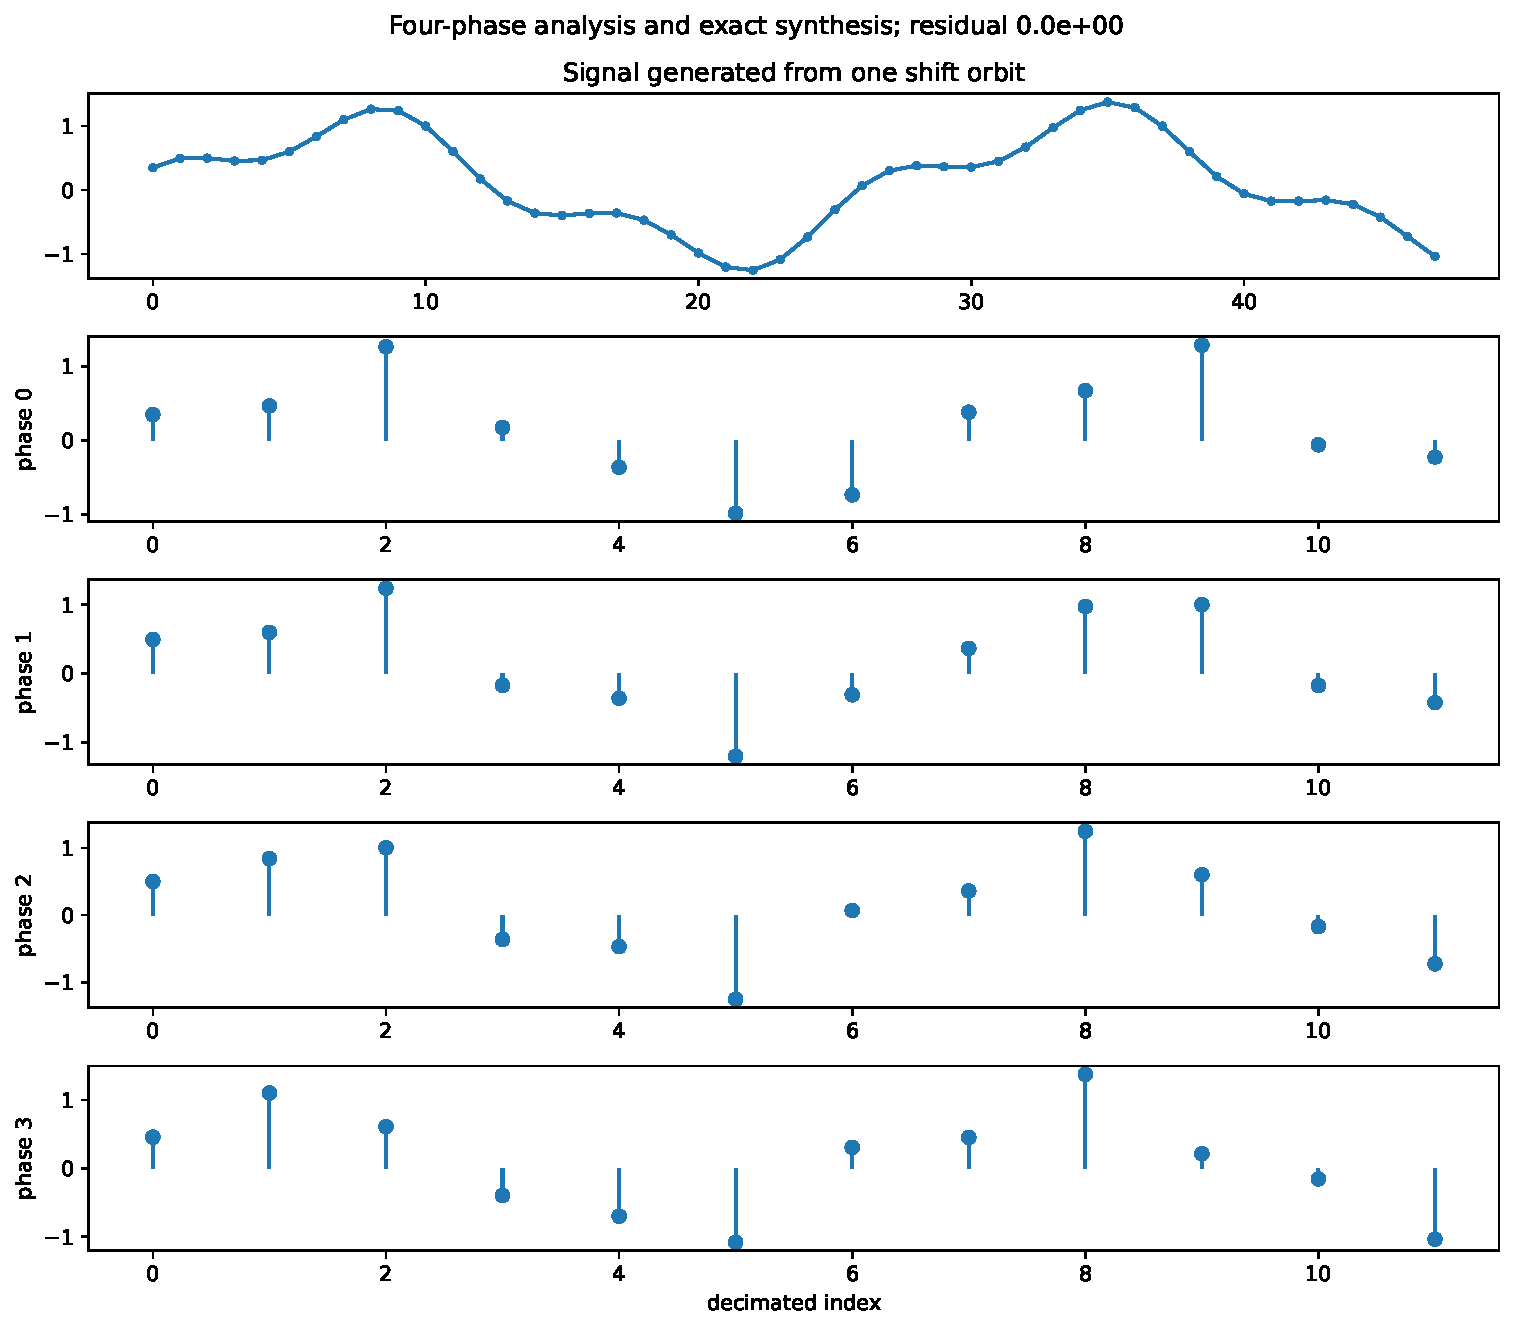
\includegraphics[width=0.94\textwidth]{01_polyphase_analysis.pdf}
\caption{Four-phase analysis of a finite signal. The channels are decimated coordinate packets; interleaving them gives the original signal exactly.}
\label{fig:polyphase-analysis}
\end{figure}

\subsection{Nested refinement}

Suppose $N\mid M$. Every coarse phase has a disjoint family of fine descendants:
\[
\operatorname{Child}_{M}(N,r)
=
\{s:0\le s<M,\ s\equiv r\pmod N\}.
\]

\begin{theorem}[Exact nested refinement]
For $N\mid M$,
\[
\boxed{
P_{N,r}
=
\sum_{\substack{0\le s<M\\s\equiv r\, (\mathrm{mod}\,N)}}P_{M,s}.
}
\]
\end{theorem}

\begin{proof}
An integer $n$ satisfies $n\equiv r\pmod N$ exactly when its unique residue $s=n\bmod M$ lies among the listed descendants. The fine indicators are disjoint, so their sum is the coarse indicator.
\end{proof}

This identity is the signal form of the refinement law introduced in Paper II. It is not merely a denser sampling rule. The coarse channel is exactly the sum of its descendants.

\section{Linear time-invariant operators as transfer matrices}

Let $h$ be a finite impulse response and
\[
y=h*x,
\qquad
y[n]=\sum_{q\in\bbZ}h[q]x[n-q].
\]
Resolve both input and output into $N$ phases. For output phase $k$ and input phase $s$, define the transfer kernel
\[
\boxed{
h_{ks}[m]=h[Nm+k-s].
}
\]
Out-of-range taps are understood to be zero.

\begin{theorem}[Exact FIR polyphase transfer law]
The output channels satisfy
\[
\boxed{
y_k[n]
=
\sum_{s=0}^{N-1}\sum_{m\in\bbZ}
h_{ks}[m]x_s[n-m].
}
\]
Equivalently, in the channel $z$-transform,
\[
\bm Y(z)=\bm H^{(N)}(z)\bm X(z),
\qquad
H^{(N)}_{ks}(z)=\sum_m h[Nm+k-s]z^{-m}.
\]
\end{theorem}

\begin{proof}
Evaluate $y$ at address $Nn+k$ and partition every input index by its residue $s$:
\[
\begin{aligned}
y[Nn+k]
&=\sum_qh[q]x[Nn+k-q]\\
&=\sum_{s=0}^{N-1}\sum_m
h[Nm+k-s]x[N(n-m)+s].
\end{aligned}
\]
The last factor is $x_s[n-m]$, giving the time-domain formula. Taking channel transforms gives the matrix formula.
\end{proof}

\begin{figure}[htbp]
\centering
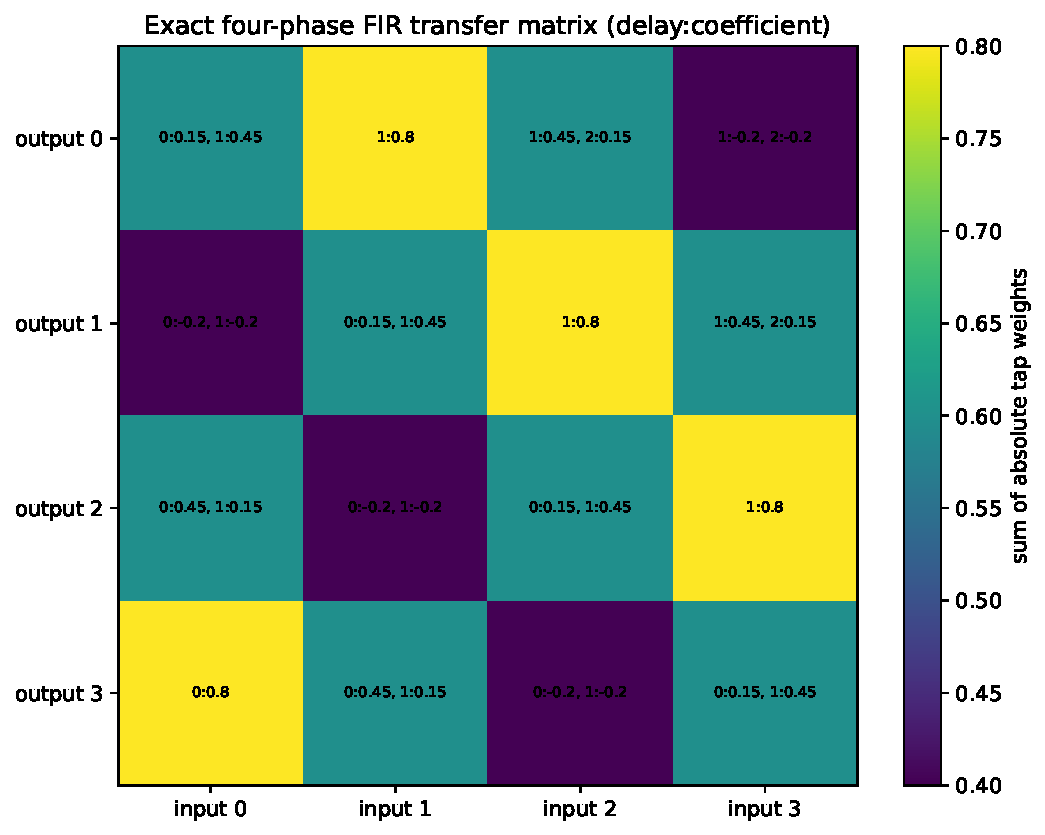
\includegraphics[width=0.80\textwidth]{02_filter_transfer_matrix.pdf}
\caption{The exact transfer matrix for a seven-tap FIR filter in four phases. Every cell records the delays and coefficients carrying one input packet into one output packet.}
\label{fig:filter-matrix}
\end{figure}

\begin{remark}[Operator-block form]
If $H$ denotes convolution by $h$, the same identity is
\[
H=\sum_{k,s}P_{N,k}HP_{N,s}.
\]
Thus the familiar polyphase matrix is exactly the transfer-block matrix of the seed calculus.
\end{remark}

\section{Analysis banks, synthesis banks, and perfect reconstruction}

Let $\bm E(z)$ be an analysis polyphase matrix and $\bm R(z)$ a synthesis matrix. The channel signal after analysis and synthesis is
\[
\widehat{\bm X}(z)=\bm R(z)\bm E(z)\bm X(z).
\]

\begin{theorem}[Perfect-reconstruction criterion]
An $N$-channel filter bank reconstructs every input up to a delay $d$ exactly when
\[
\boxed{
\bm R(z)\bm E(z)=z^{-d}I_N.
}
\]
If the right side is $c z^{-d}I_N$ with $c\ne0$, reconstruction holds up to a scalar gain and delay.
\end{theorem}

\begin{proof}
The condition is sufficient by substitution. Conversely, if every channel vector is reconstructed with delay $d$, then the linear operator $\bm R(z)\bm E(z)-z^{-d}I_N$ annihilates every channel vector, hence is the zero matrix.
\end{proof}

\subsection{The Haar bank}

The Haar analysis matrix is
\[
\bm E_{\mathrm{H}}
=
\frac1{\sqrt2}
\begin{pmatrix}
1&1\\
1&-1
\end{pmatrix}.
\]
It is orthogonal, so $\bm R_{\mathrm{H}}=\bm E_{\mathrm{H}}^{\mathsf T}$ and
\[
\bm R_{\mathrm{H}}\bm E_{\mathrm{H}}=I_2.
\]
The channels are
\[
a[n]=\frac{x[2n]+x[2n+1]}{\sqrt2},
\qquad
d[n]=\frac{x[2n]-x[2n+1]}{\sqrt2}.
\]

\begin{corollary}[Haar energy identity]
\[
\boxed{
\|x\|_2^2=\|a\|_2^2+\|d\|_2^2.
}
\]
\end{corollary}

\begin{proof}
This is Parseval's identity for the orthogonal matrix $\bm E_{\mathrm{H}}$, applied independently to every adjacent sample pair.
\end{proof}

\begin{figure}[htbp]
\centering
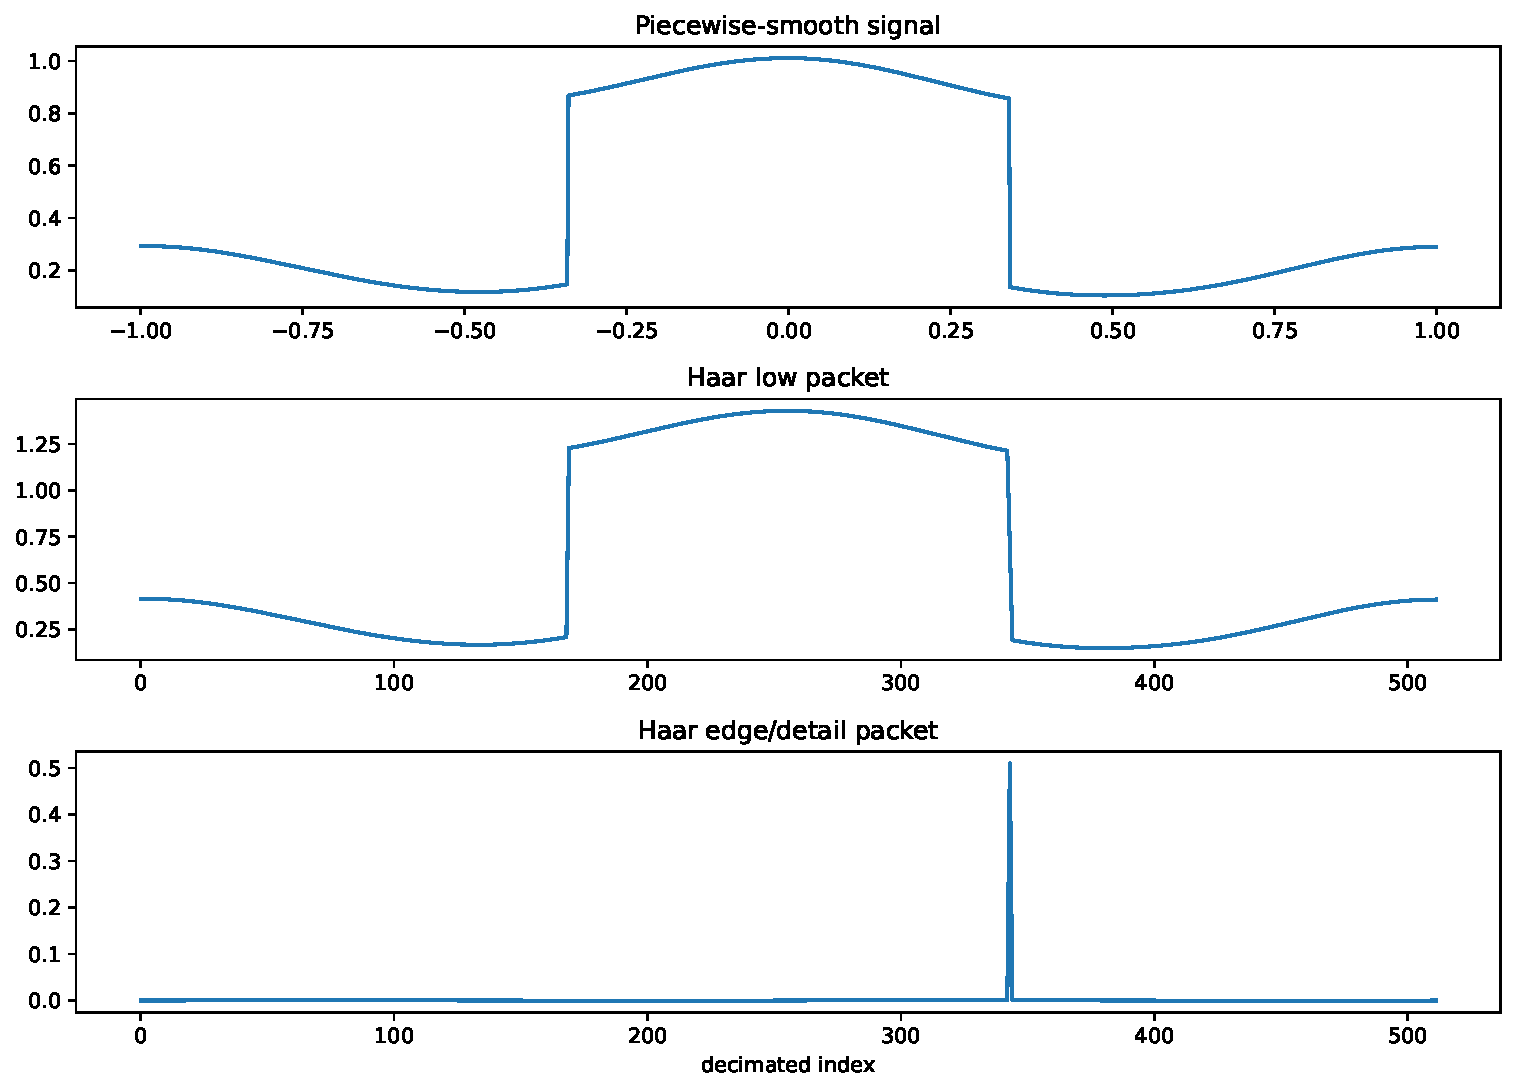
\includegraphics[width=0.92\textwidth]{03_haar_edge_packets.pdf}
\caption{A piecewise-smooth signal and its first Haar low/detail packets. The jump is concentrated in the detail channel rather than represented by a global oscillatory basis.}
\label{fig:haar-packets}
\end{figure}

\subsection{Predict--update lifting}

Split $x$ into even and odd channels $e,o$. Define
\[
d=o-e,
\qquad
s=e+\frac12d.
\]
The inverse is
\[
e=s-\frac12d,
\qquad
o=d+e.
\]

\begin{theorem}[Exact lifting reconstruction]
The predict--update map $(e,o)\mapsto(s,d)$ is invertible with determinant one and the displayed inverse. Consequently the associated finite transform reconstructs every even-length signal exactly.
\end{theorem}

\begin{proof}
The forward matrix is
\[
\begin{pmatrix}s\\d\end{pmatrix}
=
\begin{pmatrix}1/2&1/2\\-1&1\end{pmatrix}
\begin{pmatrix}e\\o\end{pmatrix},
\]
whose determinant is one. Direct substitution gives the inverse formulas.
\end{proof}

\section{Wavelet packets as addressed refinements}

Apply the Haar analysis to both children at each stage. A binary word $\alpha\in\{0,1\}^{\ell}$ addresses a depth-$\ell$ packet, denoted $W_{\ell,\alpha}x$. Appending $0$ or $1$ selects the low or high child.

\begin{theorem}[Wavelet-packet reconstruction and energy]
At every finite depth $\ell$,
\[
\boxed{
x=\sum_{\alpha\in\{0,1\}^{\ell}}W_{\ell,\alpha}^{*}W_{\ell,\alpha}x,
}
\]
and
\[
\boxed{
\|x\|_2^2
=
\sum_{\alpha\in\{0,1\}^{\ell}}
\|W_{\ell,\alpha}x\|_2^2.
}
\]
\end{theorem}

\begin{proof}
The one-level Haar map is unitary. The depth-$\ell$ transform is a composition and direct sum of unitary maps, hence unitary. The first identity is synthesis after analysis; the second is Parseval's identity.
\end{proof}

\begin{figure}[htbp]
\centering
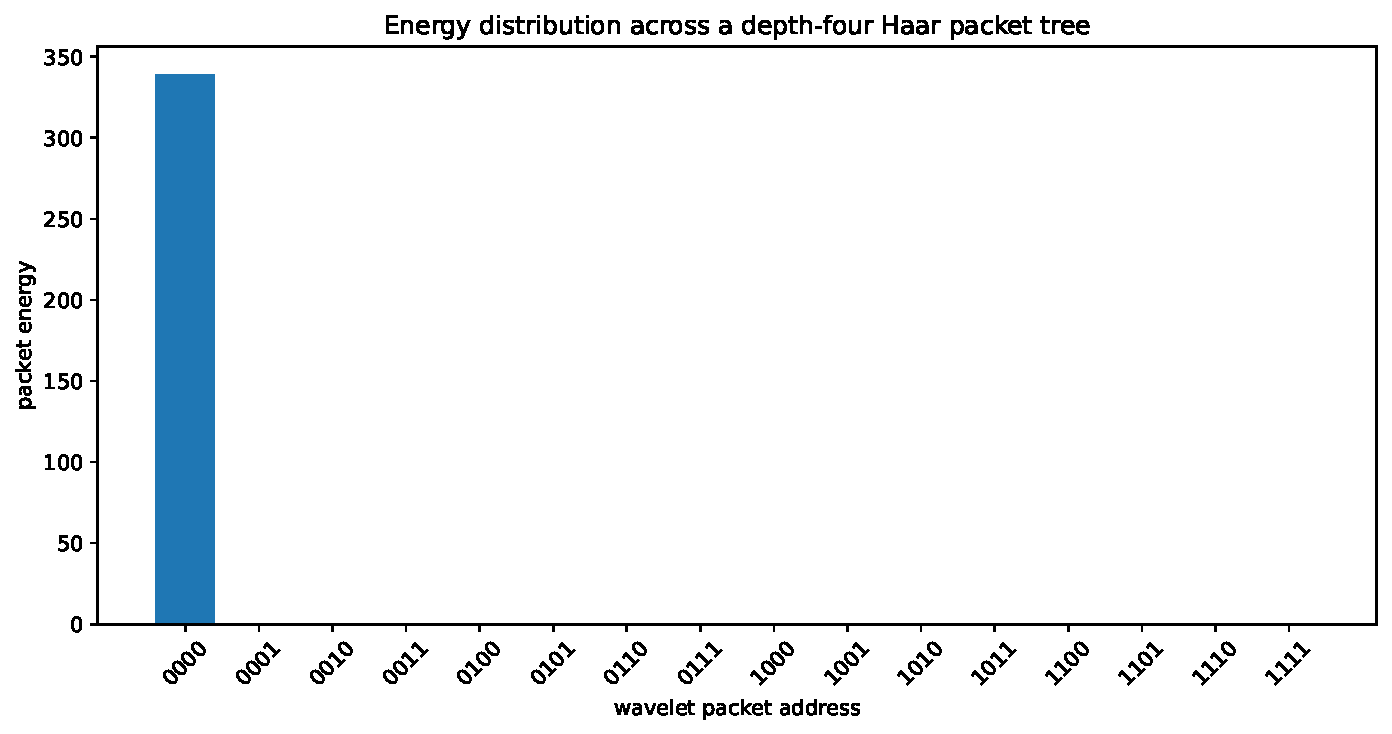
\includegraphics[width=0.92\textwidth]{04_wavelet_packet_energy.pdf}
\caption{Energy of the sixteen depth-four Haar packet addresses for the test signal. The packet address is an operator word in the common seed grammar.}
\label{fig:wavelet-energy}
\end{figure}

\begin{classical}[Wavelet boundary]
The existence and perfect-reconstruction theory of wavelets and filter banks are classical. Their role here is structural: they provide a fully developed realization in which seed generation, packet addressing, refinement, transfer blocks, and exact synthesis can all be read literally in the common operator language.
\end{classical}

\section{Known edge packets and spectral reconstruction}

The central distinction is between approximating a jump globally and retaining it as its own packet.

Let
\[
f=s+j
\]
where $s$ belongs to a smooth approximation class and $j$ is a known discontinuity packet. Let $Q_m$ be any approximation operator applied only to $s$, and define
\[
\widetilde f_m=Q_ms+j.
\]

\begin{theorem}[Exact known-edge theorem]
For every norm for which the expressions are defined,
\[
\boxed{
f-\widetilde f_m=s-Q_ms,
\qquad
\|f-\widetilde f_m\|=\|s-Q_ms\|.
}
\]
No approximation of $j$ occurs.
\end{theorem}

\begin{proof}
Subtract:
\[
f-\widetilde f_m=(s+j)-(Q_ms+j)=s-Q_ms.
\]
Taking the norm gives the second identity.
\end{proof}

\begin{corollary}[Several exact edge packets]
If
\[
f=s+\sum_{q=1}^{M}j_q
\]
and every $j_q$ is retained exactly, then
\[
\left\|f-\left(Q_ms+\sum_qj_q\right)\right\|
=\|s-Q_ms\|.
\]
Curved edges, corners, and different jump amplitudes do not alter the identity.
\end{corollary}

\begin{boundary}[What the theorem does and does not say]
The theorem explains why global ringing caused by spectrally approximating a known jump is absent from the reconstructed jump packet. It does not discover the packet. If the packet is wrong, its error is reconstructed exactly as well. Nor does the theorem prevent unrelated truncation errors in the smooth packet, domain-boundary errors, noise, or model mismatch.
\end{boundary}

\section{Mask, amplitude, and smooth-background error}

Suppose a scalar jump packet is
\[
j=a\mathbf 1_{\Omega},
\]
and an estimated packet is
\[
\widehat j=\widehat a\mathbf 1_{\widehat\Omega}.
\]

\begin{theorem}[Packet perturbation bound]
For $1\le p<\infty$,
\[
\boxed{
\|j-\widehat j\|_{L^p}
\le
|a-\widehat a|\,\mu(\Omega)^{1/p}
+
|\widehat a|\,\mu(\Omega\triangle\widehat\Omega)^{1/p}.
}
\]
For $p=\infty$,
\[
\|j-\widehat j\|_{\infty}
\le |a-\widehat a|+|\widehat a|\,
\mathbf 1_{\Omega\triangle\widehat\Omega\ne\varnothing}.
\]
\end{theorem}

\begin{proof}
Write
\[
a\mathbf 1_{\Omega}-\widehat a\mathbf 1_{\widehat\Omega}
=(a-\widehat a)\mathbf 1_{\Omega}
+\widehat a(\mathbf 1_{\Omega}-\mathbf 1_{\widehat\Omega}).
\]
Apply the triangle inequality and use
\[
\|\mathbf 1_{\Omega}-\mathbf 1_{\widehat\Omega}\|_{L^p}
=\mu(\Omega\triangle\widehat\Omega)^{1/p}.
\]
The supremum bound follows in the same way.
\end{proof}

If $\widehat s$ is an estimated smooth packet, then
\[
\boxed{
\|f-(\widehat s+\widehat j)\|_p
\le
\|s-\widehat s\|_p
+|a-\widehat a|\mu(\Omega)^{1/p}
+|\widehat a|\mu(\Omega\triangle\widehat\Omega)^{1/p}.
}
\]
This is the correct separation of errors. Detection error is not hidden inside a generic reconstruction score.

\begin{conjecture}[Stable edge-packet recovery]
For specified piecewise-smooth classes, contrast bounds, separation conditions, and noise models, there should exist a multiscale packet estimator whose symmetric-difference error and amplitude error converge at rates controlled independently of the smooth approximation rate. A theorem of this kind would turn the conditional known-edge result into a stable data-driven reconstruction theorem. No universal version is asserted here.
\end{conjecture}

\section{One-dimensional numerical study}

The one-dimensional signal contains a smooth non-bandlimited background and a positive rectangular packet. Three reconstructions are compared:

\begin{enumerate}[label=(\roman*)]
\item global Fourier truncation of the complete signal;
\item Fourier truncation of the known smooth packet plus the exact jump packet;
\item a two-class estimated packet followed by harmonic background filling, spectral smoothing, and jump-amplitude estimation.
\end{enumerate}

\begin{figure}[htbp]
\centering
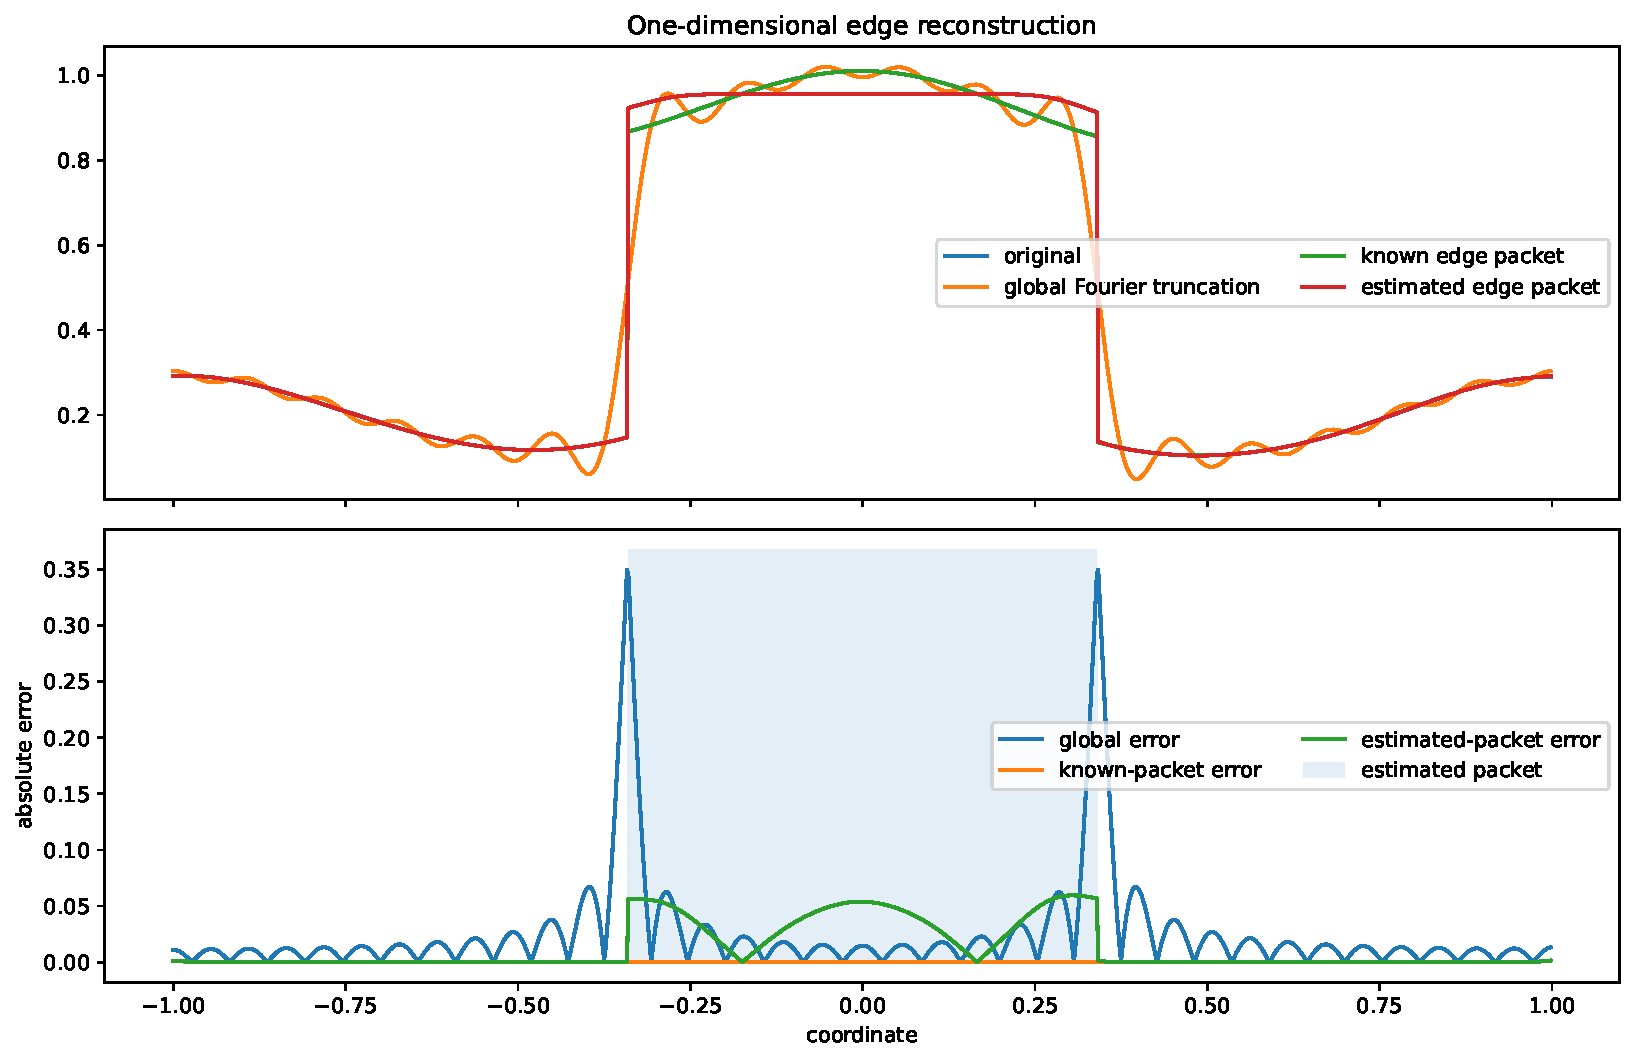
\includegraphics[width=0.98\textwidth]{05_edge_reconstruction_1d.pdf}
\caption{One-dimensional reconstruction and absolute error. The known packet removes the edge from the global spectral approximation. The estimated packet is visibly better than the global reconstruction in this limited test but retains smooth-background estimation error.}
\label{fig:edge-1d}
\end{figure}

\begin{certificate}[One-dimensional errors]
With eighteen retained modes, the measured values were
\[
\begin{array}{lrr}
\toprule
\text{method}&\RMSE&\text{maximum absolute error}\\
\midrule
\text{global Fourier truncation}&5.4023\times10^{-2}&3.4968\times10^{-1}\\
\text{known edge packet}&1.3692\times10^{-4}&1.4503\times10^{-3}\\
\text{estimated edge packet}&2.4029\times10^{-2}&5.9530\times10^{-2}\\
\bottomrule
\end{array}
\]
The simple estimator recovered the binary mask exactly in this deliberately separated two-class example. That result is a property of this test, not a universal guarantee.
\end{certificate}

\begin{figure}[htbp]
\centering
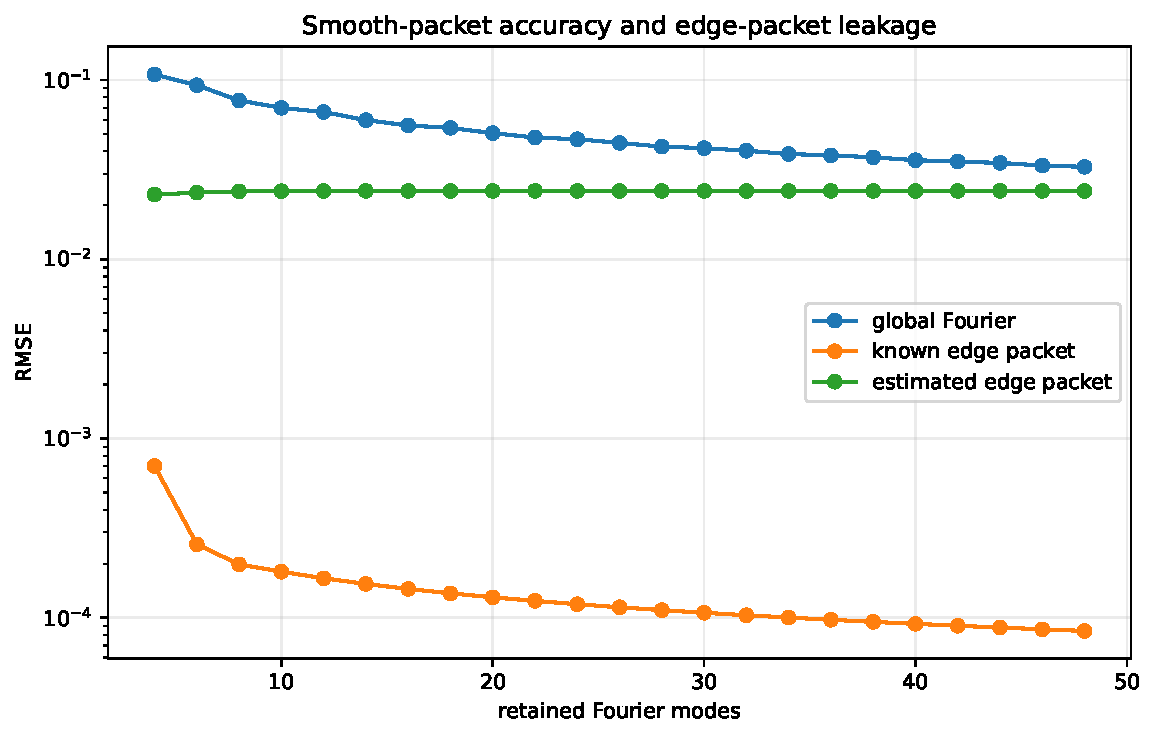
\includegraphics[width=0.84\textwidth]{06_edge_error_vs_resolution.pdf}
\caption{Error as spectral resolution increases. The known packet follows only the smooth approximation error. The estimated reconstruction reaches a floor determined by background and amplitude estimation.}
\label{fig:edge-resolution}
\end{figure}

\section{Two-dimensional edge packets}

The first image consists of a smooth background and one sharp disk. The same three logical levels must remain separate:

\begin{enumerate}[label=(\alph*)]
\item the exact theorem using the known decomposition;
\item a limited estimator designed for a positive-contrast two-class packet;
\item the open problem of recovering arbitrary edge packets under noise and model ambiguity.
\end{enumerate}

\begin{figure}[htbp]
\centering
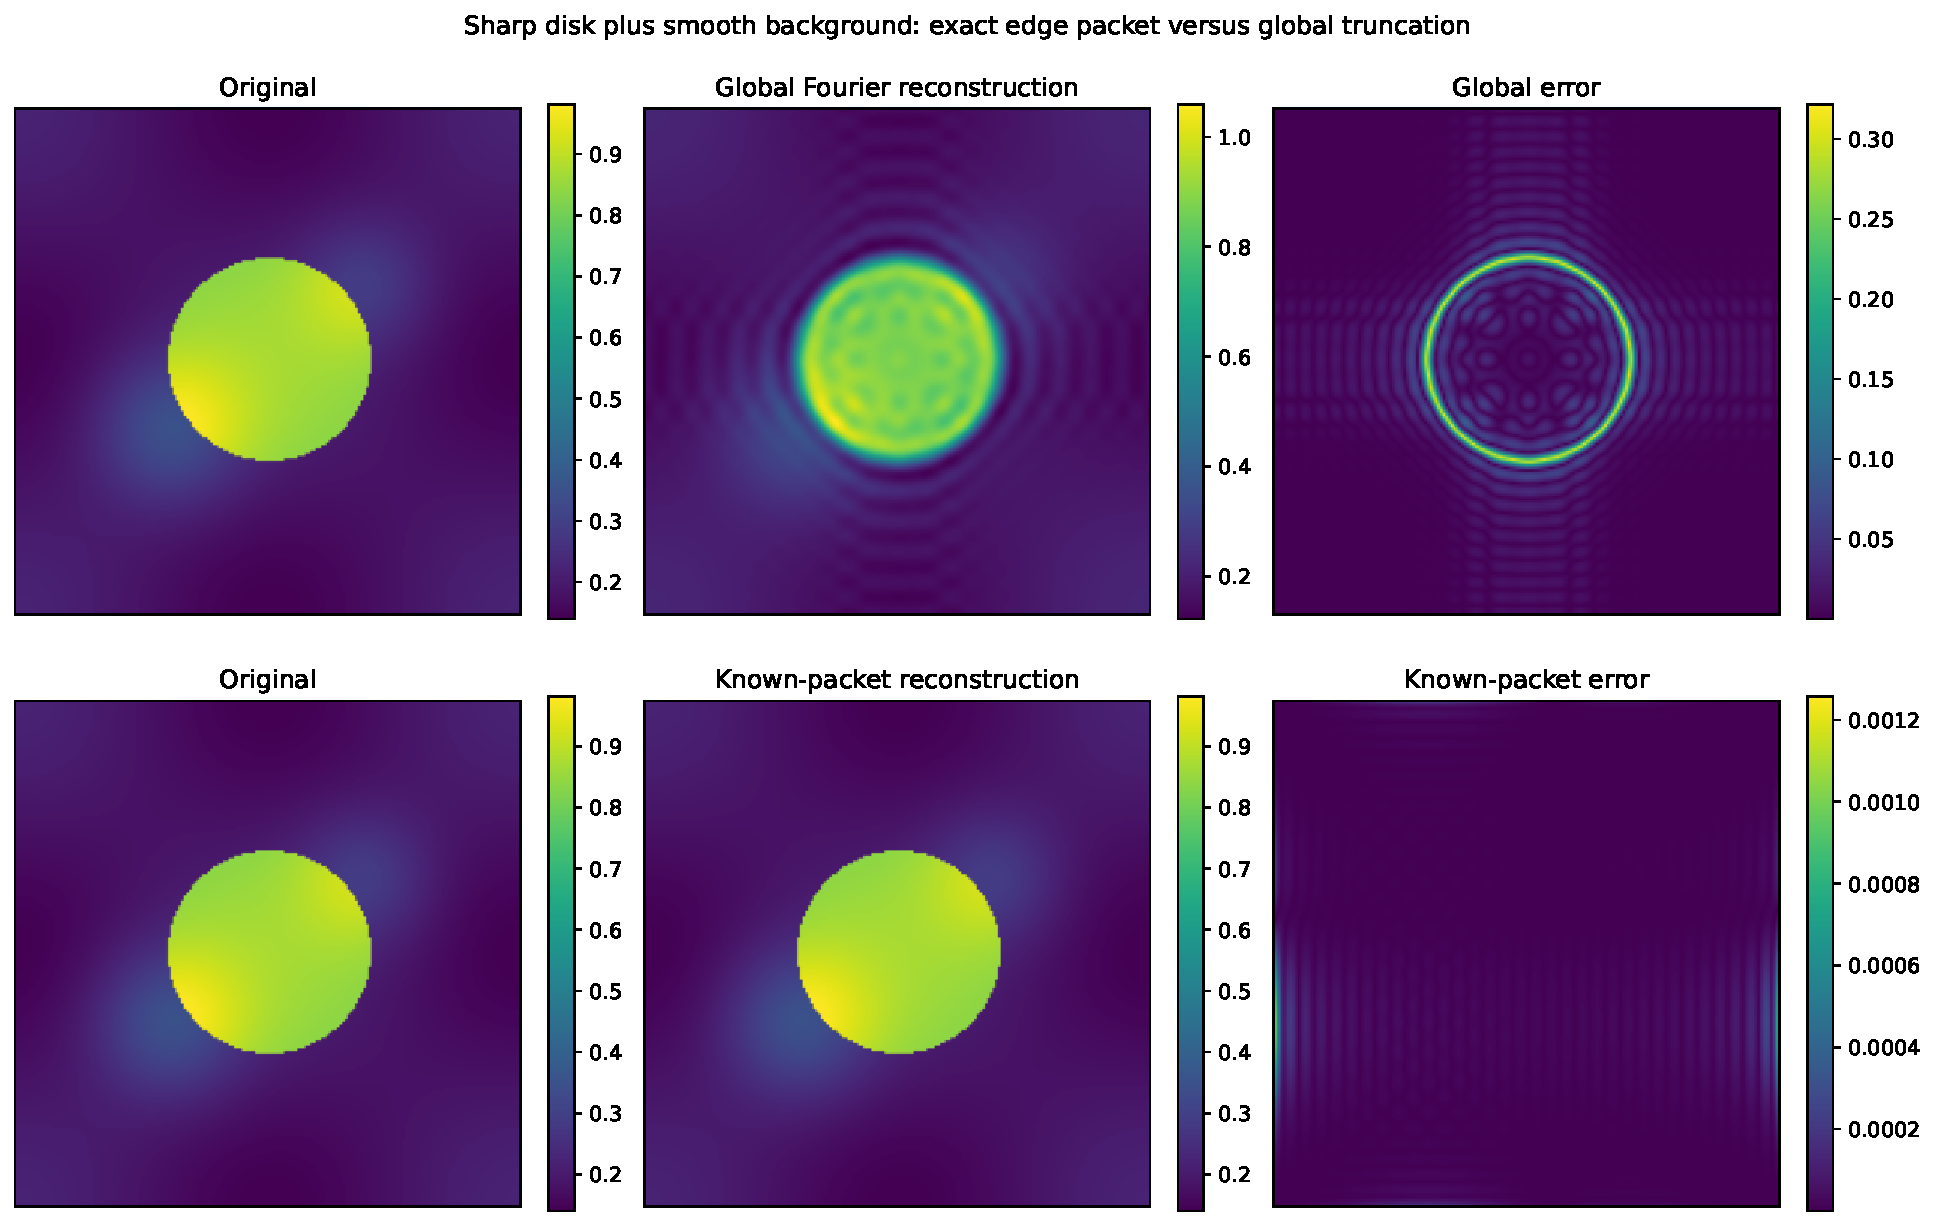
\includegraphics[width=0.99\textwidth]{07_known_edge_packet_2d.pdf}
\caption{A sharp disk on a smooth background. Global Fourier truncation produces a bright boundary halo and oscillatory interior and exterior error. Retaining the exact edge packet leaves only the smooth-background approximation error.}
\label{fig:known-2d}
\end{figure}

\begin{certificate}[Two-dimensional errors]
For the disk experiment,
\[
\begin{array}{lrr}
\toprule
\text{method}&\text{full-image RMSE}&\text{boundary-band RMSE}\\
\midrule
\text{global Fourier truncation}&3.7643\times10^{-2}&1.8541\times10^{-1}\\
\text{known edge packet}&6.4752\times10^{-5}&1.2709\times10^{-5}\\
\text{estimated edge packet}&3.4043\times10^{-3}&8.8834\times10^{-3}\\
\bottomrule
\end{array}
\]
The mask intersection-over-union was one in this positive-contrast synthetic case. The amplitude was estimated rather than inserted from the generating model.
\end{certificate}

\begin{figure}[htbp]
\centering
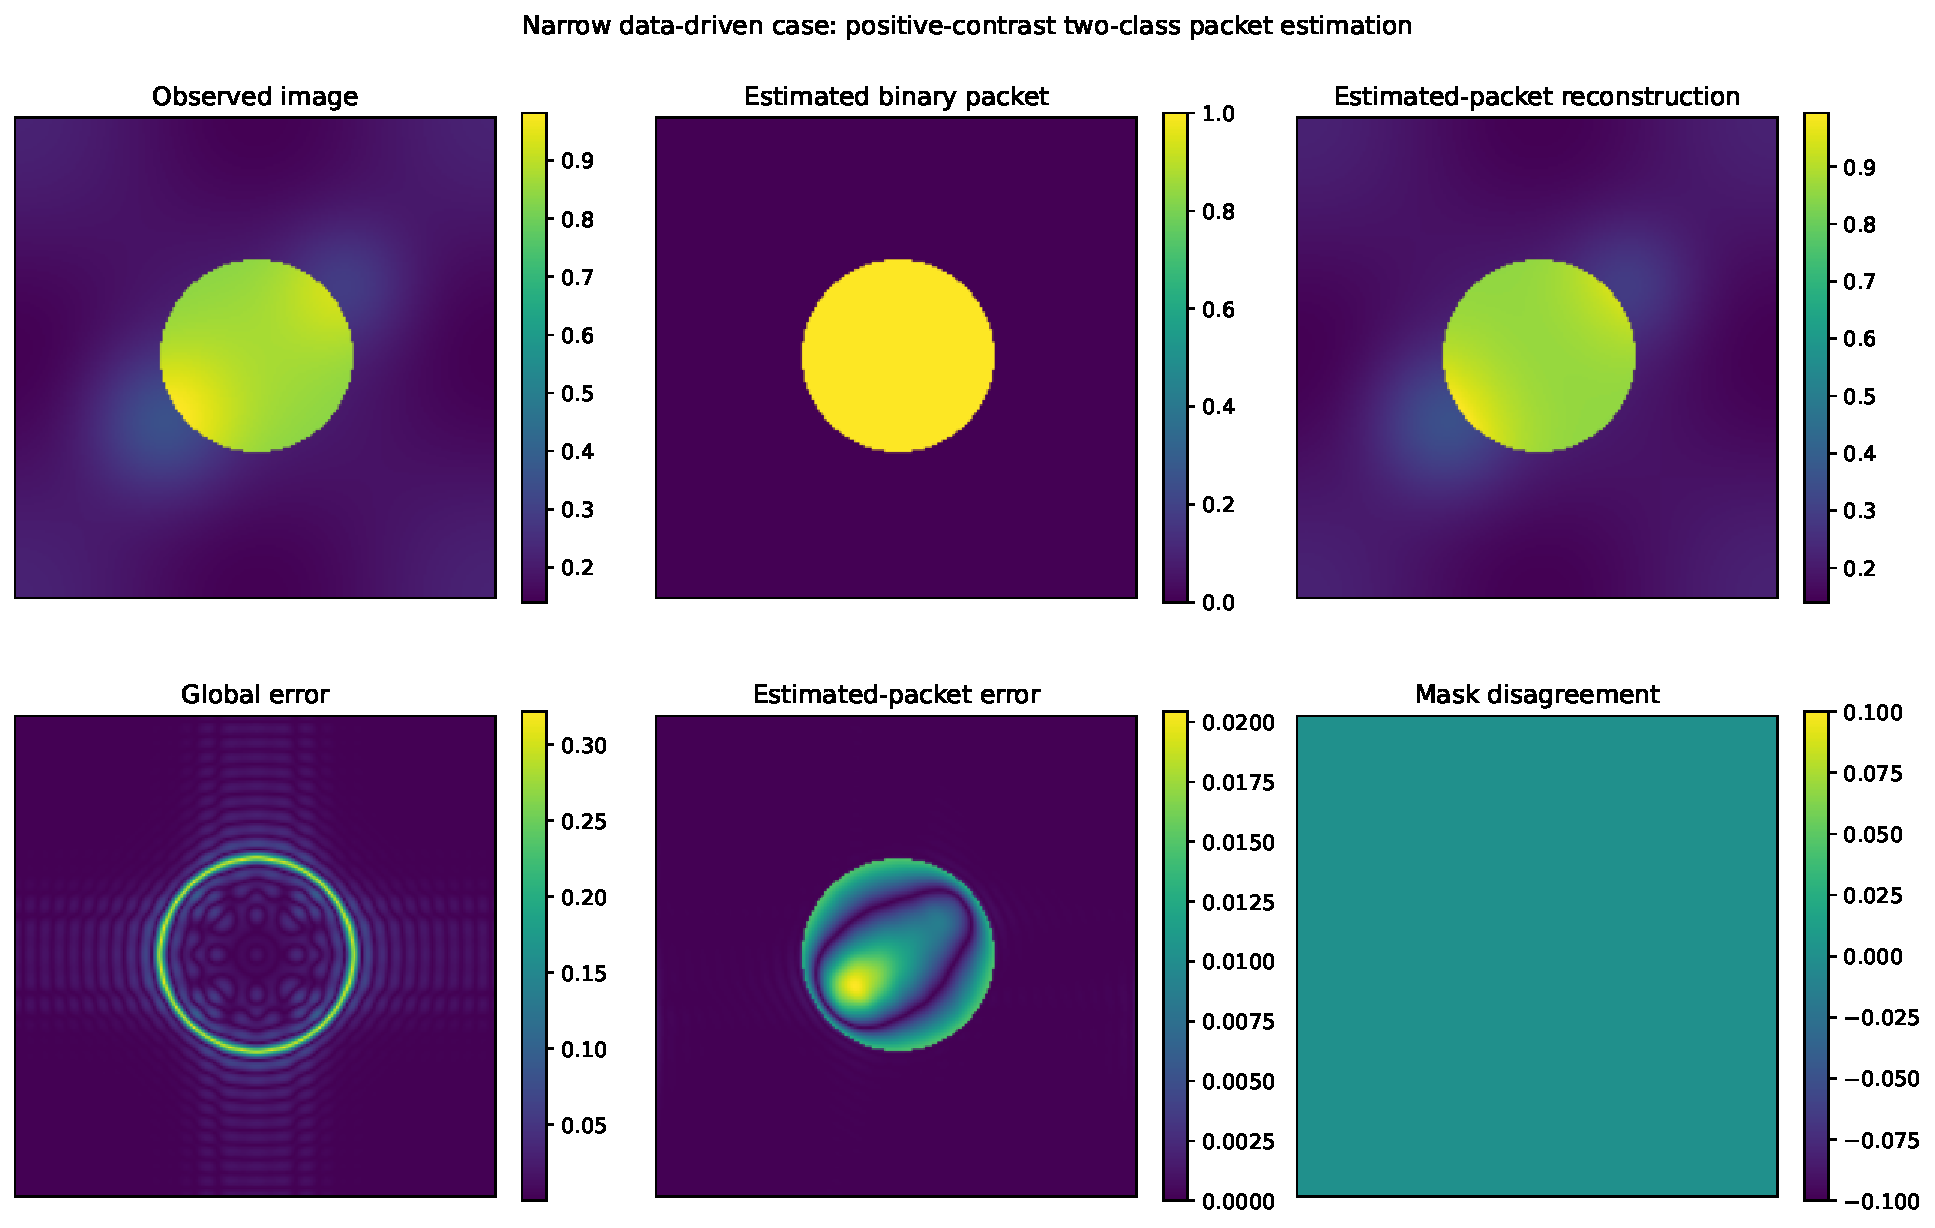
\includegraphics[width=0.99\textwidth]{08_estimated_edge_packet_2d.pdf}
\caption{The limited data-driven experiment. The observed image alone is thresholded into two intensity classes, cleaned topologically, harmonically filled, spectrally smoothed, and recombined with an estimated jump.}
\label{fig:estimated-2d}
\end{figure}

\subsection{Curves, corners, and multiple amplitudes}

The exact theorem does not depend on the shape of the known edge packet. The next experiment contains a disk, a square, and a diamond with different jump amplitudes.

\begin{figure}[htbp]
\centering
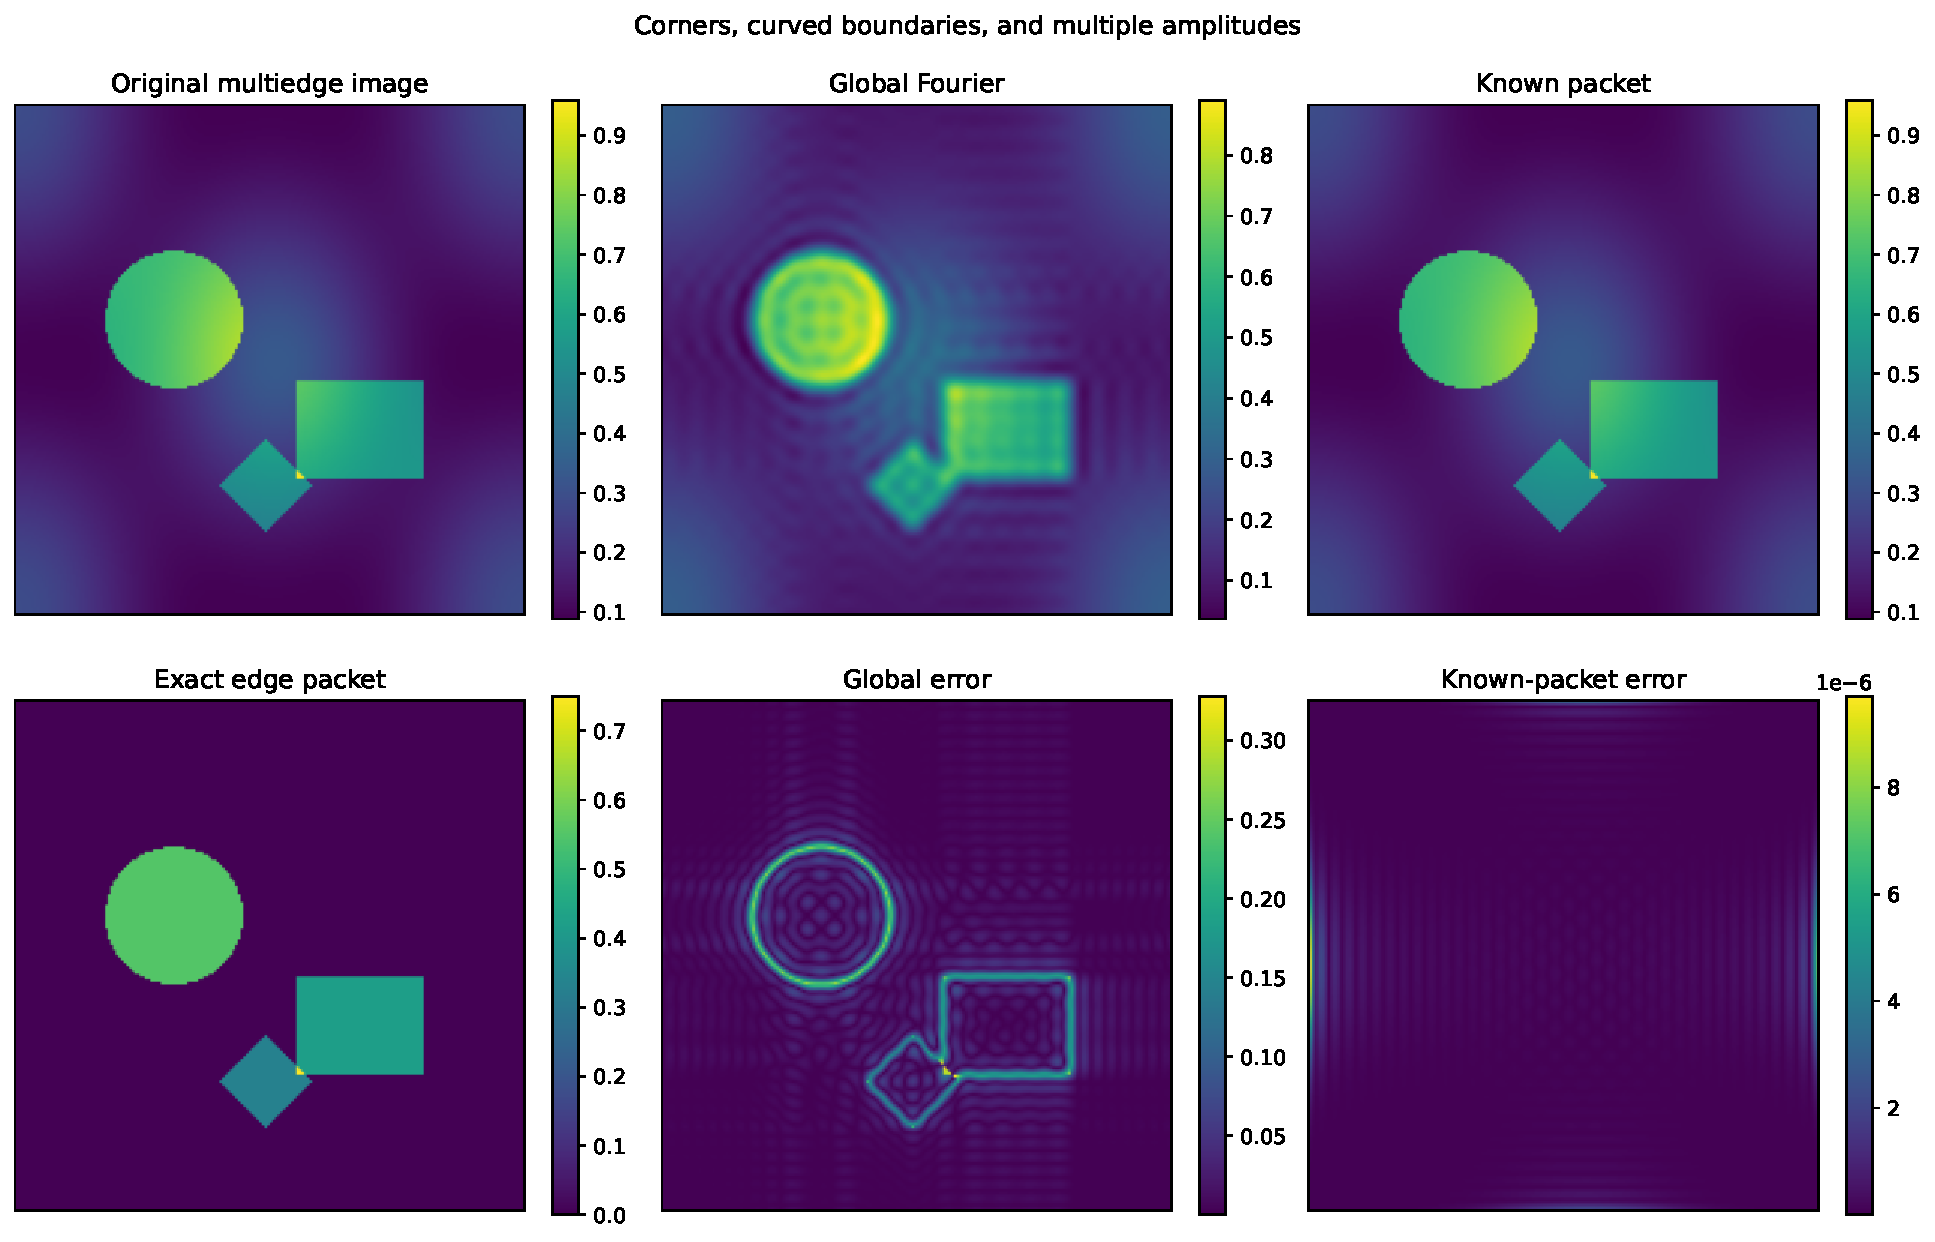
\includegraphics[width=0.99\textwidth]{09_multiedge_stress_test.pdf}
\caption{Known-packet stress test with curved boundaries, corners, overlap, and different jump amplitudes. The exact packet is not a binary mask multiplied by one amplitude; it is the complete piecewise packet.}
\label{fig:multiedge}
\end{figure}

\begin{certificate}[Multiedge errors]
The global reconstruction had RMSE $3.3740\times10^{-2}$ and maximum error $3.2807\times10^{-1}$. The known-packet reconstruction had only the remaining smooth-background error. The experiment verifies the theorem for a composite packet; it is not a data-driven multiregion segmentation result.
\end{certificate}

\section{Sparse wavelet packets and global Fourier modes}

A sharp edge is spatially local but spectrally global. Wavelets often provide a more economical coordinate system once enough localized coefficients are retained. To keep the comparison explicit, the numerical study keeps the largest coefficients in a fixed depth-five Haar packet basis and compares them with the same number of largest Fourier coefficients.

\begin{figure}[htbp]
\centering
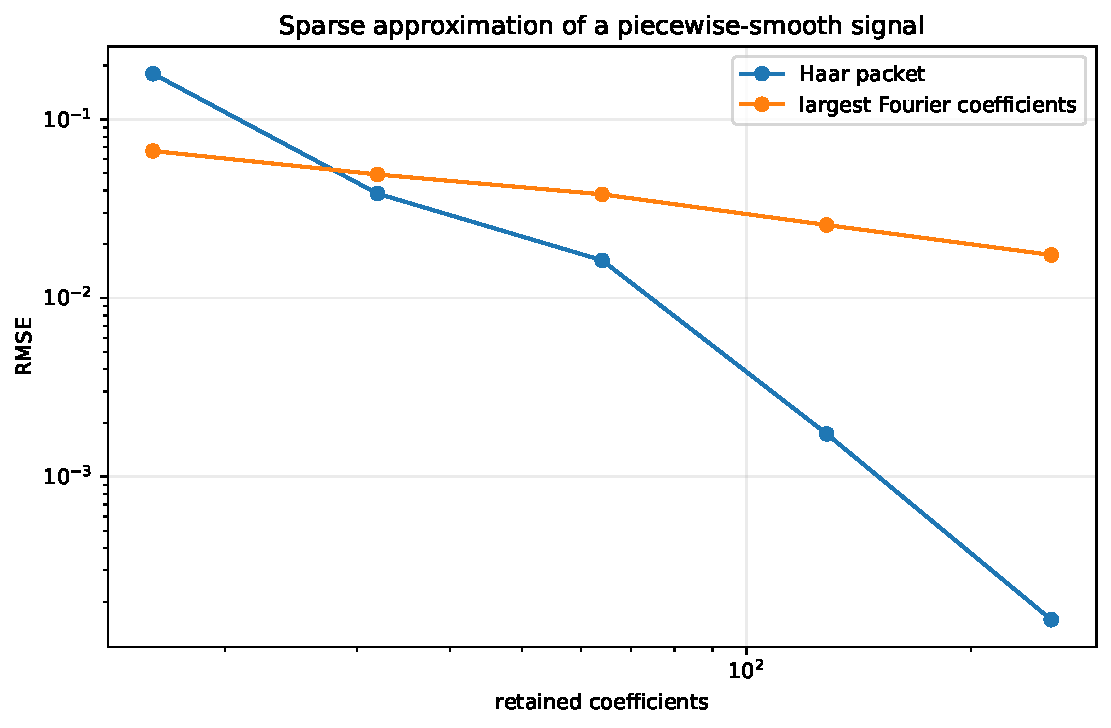
\includegraphics[width=0.83\textwidth]{10_sparse_wavelet_fourier.pdf}
\caption{Sparse approximation of the test signal. With very few coefficients the global Fourier basis is initially better; after the edge packets are resolved, the Haar packet error decays much faster in this example.}
\label{fig:sparse-comparison}
\end{figure}

\begin{table}[htbp]
\centering
\caption{Sparse approximation errors for the one-dimensional test signal.}
\begin{tabular}{rrr}
\toprule
\text{retained coefficients}&\text{Haar packet RMSE}&\text{Fourier RMSE}\\
\midrule
16&$1.7999\times10^{-1}$&$6.6522\times10^{-2}$\\
32&$3.8414\times10^{-2}$&$4.9153\times10^{-2}$\\
64&$1.6267\times10^{-2}$&$3.8056\times10^{-2}$\\
128&$1.7387\times10^{-3}$&$2.5631\times10^{-2}$\\
256&$1.5870\times10^{-4}$&$1.7424\times10^{-2}$\\
\bottomrule
\end{tabular}
\label{tab:sparse}
\end{table}

\begin{boundary}[Basis selection]
This table compares two fixed finite coordinate systems for one signal. It does not prove that Haar packets are optimal, that Fourier is inferior on smooth or oscillatory data, or that a single packet tree is best for every edge geometry. The point is that the seed calculus records both systems with the same analysis, transfer, refinement, and synthesis maps.
\end{boundary}

\section{Finite adaptive packet trees}

The preceding sparse comparison used one fixed depth-five packet basis.  A refinement tree permits a stronger choice: different branches may stop at different depths while the selected packets still form one complete coordinate system.

\begin{definition}[Complete packet pruning]
Let $\mathcal T$ be a finite rooted refinement tree.  Every node $v$ carries a projector $P_v$, the root satisfies $P_{\varnothing}=I$, and every internal node satisfies
\[
P_v=\sum_{u\in\operatorname{ch}(v)}P_u,
\qquad
P_uP_w=0\quad(u\ne w\text{ in }\operatorname{ch}(v)).
\]
A set $\Lambda$ of nodes is a complete pruning if it is an antichain and every root-to-terminal path meets $\Lambda$ exactly once.
\end{definition}

\begin{theorem}[Exact synthesis from every complete pruning]
For every complete pruning $\Lambda$,
\[
\boxed{\sum_{v\in\Lambda}P_v=I,}
\qquad
\boxed{x=\sum_{v\in\Lambda}P_vx.}
\]
Thus changing the selected tree changes the coordinates but does not introduce reconstruction error.
\end{theorem}

\begin{proof}
Starting from the root identity $P_{\varnothing}=I$, replace every unselected internal node by the exact sum of its children.  Because the tree is finite, this substitution terminates precisely at the nodes of $\Lambda$.  Pairwise annihilation of siblings shows that no component is counted twice.  Applying the resulting identity to $x$ gives the synthesis formula.
\end{proof}

Let $y$ denote the observed data.  For a complete pruning $\Lambda$, consider any finite criterion
\[
J_y(\Lambda)
=
R_y(\Lambda)
+\eta L_y(\Lambda)
+\tau K(\Lambda),
\]
where $R_y$ is a representation cost, $L_y$ is a cross-packet leakage cost, and $K$ is a tree-complexity penalty.  No additivity is needed for the first theorem.

\begin{theorem}[Finite globally optimal stable selector]
Let $\mathfrak P(\mathcal T)$ be the finite set of complete prunings of $\mathcal T$.

\begin{enumerate}[label=(\roman*)]
\item A global minimizer
\[
\Lambda_y^*\in\operatorname*{argmin}_{\Lambda\in\mathfrak P(\mathcal T)}J_y(\Lambda)
\]
always exists.
\item If the minimizer is unique, its gap
\[
\Gamma_y
=
\min_{\Lambda\ne\Lambda_y^*}
\bigl(J_y(\Lambda)-J_y(\Lambda_y^*)\bigr)
\]
is strictly positive.
\item If new data $y'$ satisfy
\[
\sup_{\Lambda\in\mathfrak P(\mathcal T)}
|J_{y'}(\Lambda)-J_y(\Lambda)|
<\frac{\Gamma_y}{2},
\]
then $\Lambda_{y'}^*=\Lambda_y^*$.
\item Every selected minimizer preserves the exact synthesis identity of the preceding theorem.
\end{enumerate}
\end{theorem}

\begin{proof}
The set of complete prunings is finite, so the minimum is attained.  A unique minimum in a finite set has a positive distance from the second-smallest value.  For any competing pruning $\Lambda\ne\Lambda_y^*$,
\[
\begin{aligned}
J_{y'}(\Lambda)-J_{y'}(\Lambda_y^*)
&\ge
J_y(\Lambda)-J_y(\Lambda_y^*)
-2\sup_{\Xi}|J_{y'}(\Xi)-J_y(\Xi)|\\
&>\Gamma_y-\Gamma_y=0.
\end{aligned}
\]
Hence the same pruning remains uniquely optimal.  Exact synthesis depends only on completeness of the pruning, not on the cost used to select it.
\end{proof}

For tree-local costs, the optimum can be found without enumerating all prunings.

\begin{theorem}[Dynamic-programming best packet basis]
Suppose
\[
J_y(\Lambda)=\sum_{v\in\Lambda}c_v(y).
\]
For a node $v$, define recursively
\[
V_y(v)
=
\begin{cases}
c_v(y),&v\text{ terminal},\\[2mm]
\displaystyle
\min\left\{c_v(y),\sum_{u\in\operatorname{ch}(v)}V_y(u)\right\},
&v\text{ internal}.
\end{cases}
\]
Stopping at $v$ when the first term is smaller and refining when the second term is smaller produces a globally optimal complete pruning.  The computation uses one comparison per internal node and therefore has cost $O(|\mathcal T|)$.
\end{theorem}

\begin{proof}
Proceed upward from the terminal nodes.  Every complete pruning below an internal node $v$ has exactly two possible forms: it either stops at $v$, with cost $c_v(y)$, or it refines and is the union of complete child prunings, whose minimum total cost is the sum of the already computed child minima.  The recursion therefore gives the exact minimum on every subtree, in particular at the root.
\end{proof}

\begin{corollary}[Local perturbation certificate]
Assume
\[
|c_v(y')-c_v(y)|\le\varepsilon_v.
\]
Define
\[
E(v)
=
\begin{cases}
\varepsilon_v,&v\text{ terminal},\\[1mm]
\displaystyle
\max\left\{\varepsilon_v,
\sum_{u\in\operatorname{ch}(v)}E(u)\right\},&v\text{ internal}.
\end{cases}
\]
Then every complete-pruning cost changes by at most $E(\varnothing)$.  Consequently,
\[
\boxed{\Gamma_y>2E(\varnothing)}
\]
is a deterministic certificate that the globally optimal pruning is unchanged.  If a noise model supplies the local bounds with probability at least $1-\delta$, the same selector is recovered with probability at least $1-\delta$.
\end{corollary}

\begin{proof}
For any pruning of the subtree rooted at $v$, either $v$ itself is selected, producing perturbation at most $\varepsilon_v$, or the pruning is the disjoint union of child prunings, producing perturbation at most the sum of the child envelopes.  The recursion therefore bounds the supremum over all subtree prunings.  The global statement follows from the gap theorem.
\end{proof}

\begin{figure}[htbp]
\centering
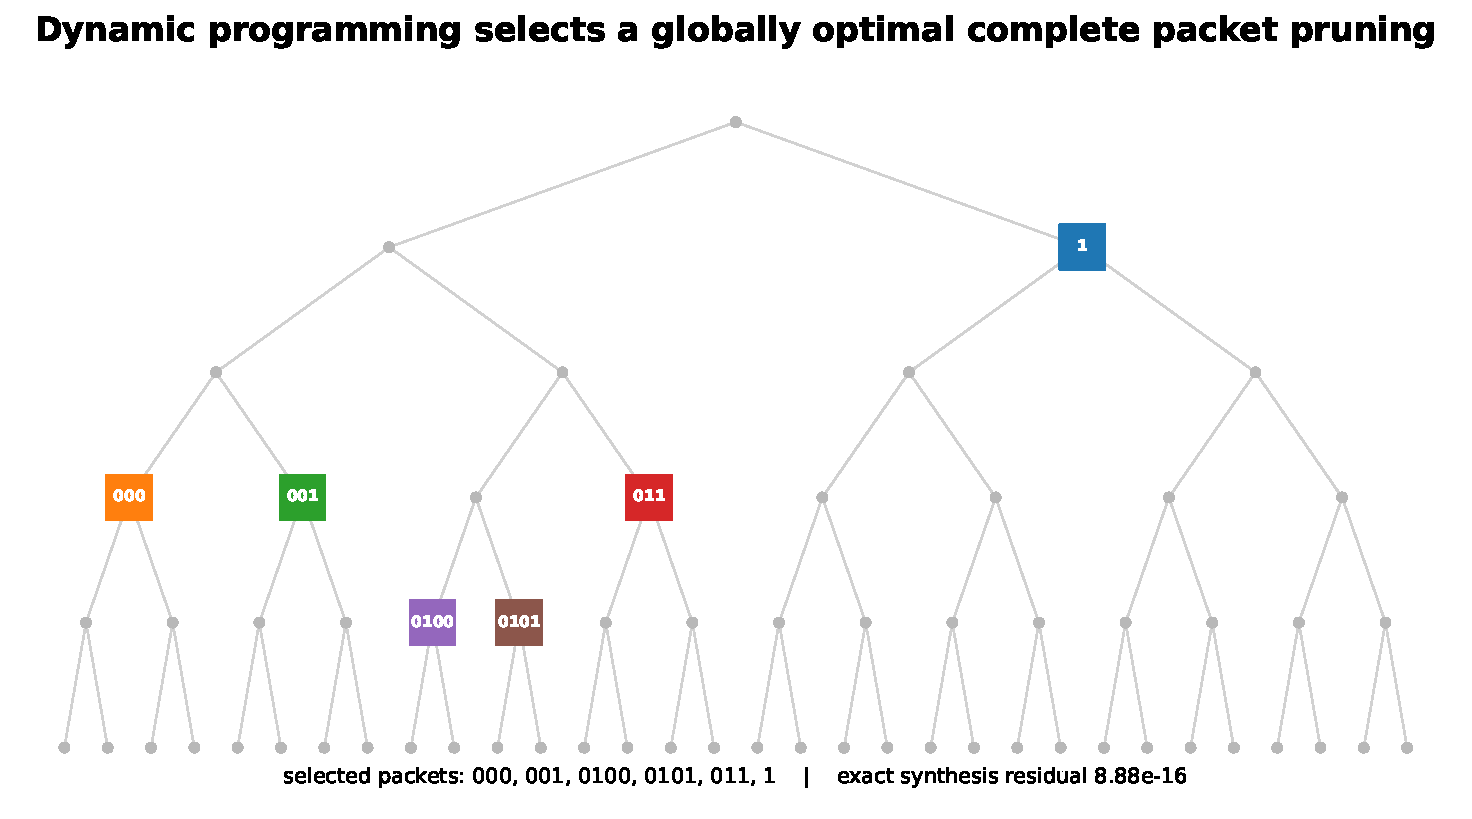
\includegraphics[width=0.97\textwidth]{17_adaptive_packet_tree.pdf}
\caption{A globally optimal mixed-depth Haar packet pruning.  The selected antichain covers the full tree, so its synthesis is exact even though different branches stop at different depths.}
\label{fig:adaptive-tree}
\end{figure}

\begin{figure}[htbp]
\centering
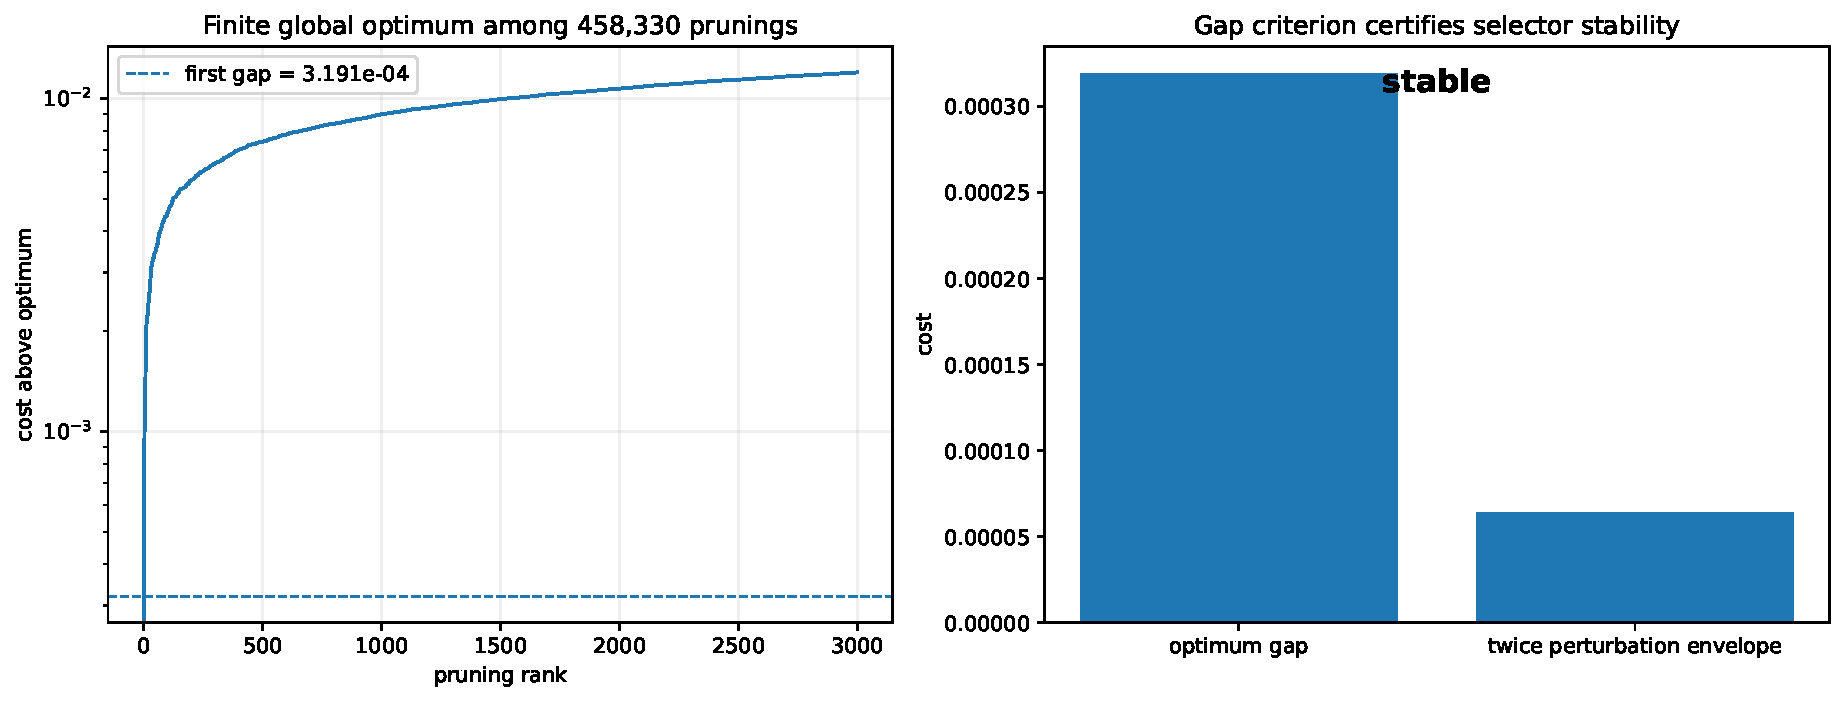
\includegraphics[width=0.97\textwidth]{18_adaptive_tree_stability.pdf}
\caption{The dynamic-programming optimum agrees with exhaustive enumeration.  A positive gap larger than twice the declared perturbation envelope certifies that the selected tree is stable.}
\label{fig:adaptive-stability}
\end{figure}

\begin{certificate}[Adaptive-tree optimum]
For the depth-five example, the complete binary tree has $458{,}330$ admissible prunings.  Dynamic programming and exhaustive enumeration returned the same minimum with residual $0$.  The selected pruning was
\[
\{000,001,0100,0101,011,1\},
\]
and mixed-depth synthesis reconstructed the signal with maximum residual $8.88\times10^{-16}$.  The optimum gap was $3.1909\times10^{-4}$, while twice the declared perturbation envelope was $6.4\times10^{-5}$, so the finite selector is certified stable.
\end{certificate}

\begin{boundary}[Finite versus asymptotic selection]
The theorem resolves the finite adaptive-tree existence, exact-synthesis, global-optimality, and margin-stability problem.  It does not by itself prove minimax rates, statistical consistency on an infinite tree, or a universal choice of representation and leakage costs for every signal class.
\end{boundary}


\section{Nonlinear signal packets}

Linear time invariance is not required for exact packet coordinates. Let a formal or analytic signal representation be
\[
A(z)=\sum_{n\ge0}a_nz^n,
\qquad
A_i=P_{N,i}A.
\]
For another representation $B(z)$, multiplication gives a nonlinear or bilinear interaction.

\begin{theorem}[Cyclic product law]
\[
\boxed{
P_{N,k}(AB)
=
\sum_{i+j\equiv k\, (\mathrm{mod}\,N)}A_iB_j.
}
\]
For the $q$th power,
\[
P_{N,k}(A^q)
=
\sum_{i_1+\cdots+i_q\equiv k}
A_{i_1}\cdots A_{i_q}.
\]
\end{theorem}

\begin{proof}
Every coefficient in $A_iB_j$ has degree congruent to $i+j$ modulo $N$. Sorting all products by their resulting residue gives the first identity. Repetition proves the power identity.
\end{proof}

\begin{figure}[htbp]
\centering
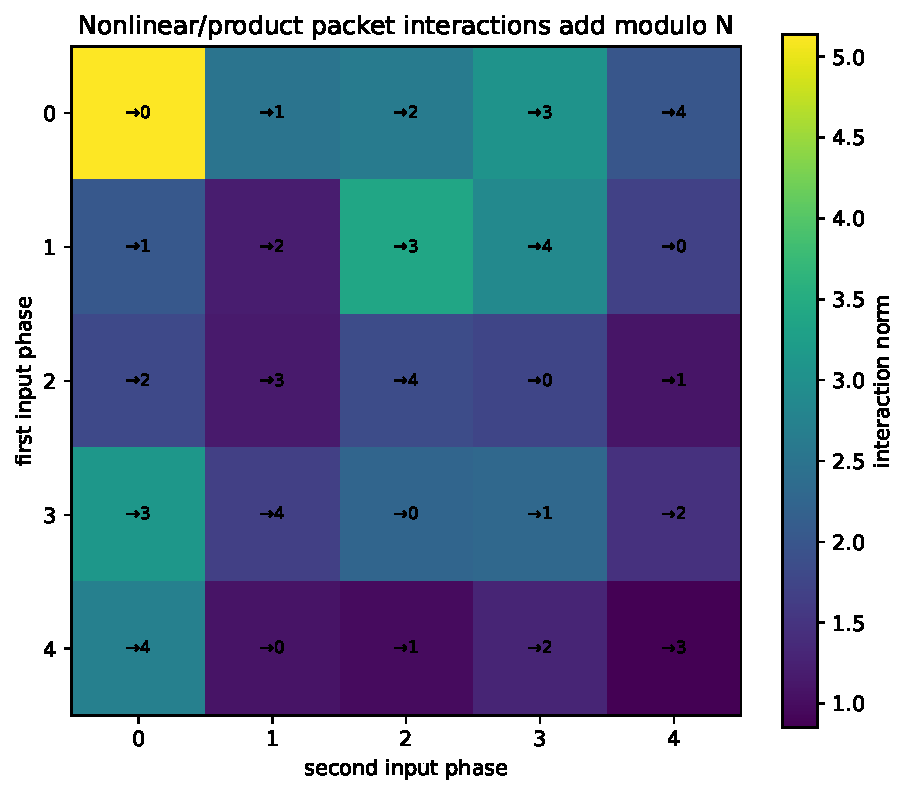
\includegraphics[width=0.76\textwidth]{14_nonlinear_phase_coupling.pdf}
\caption{Norms of pairwise product interactions for five residue phases. The label in each cell gives the output phase $(i+j)\bmod5$.}
\label{fig:nonlinear-coupling}
\end{figure}

For a finite nonlinear shift operator
\[
F(x)[n]=x[n]+\alpha x[n]x[n-1],
\]
the exact packet coordinates are simply
\[
F_r((x_s)_s)=P_{N,r}F\!\left(\sum_sP_{N,s}x\right).
\]
Analysis followed by this packet system and synthesis reproduces the direct nonlinear output exactly. The numerical residual in the companion implementation was zero to machine representation.

\section{Smith coordinates as cyclic signal coordinates}

Let $Z_0>0$ be a reference impedance and
\[
z=\frac{Z}{Z_0}=r+\ii x.
\]
The reflection coefficient is
\[
\boxed{
\Gam=\frac{z-1}{z+1},
\qquad
z=\frac{1+\Gam}{1-\Gam}.
}
\]

\begin{classical}[Cayley geometry]
The map sends the passive half-plane $r\ge0$ to the closed unit disk $|\Gam|\le1$. Constant resistance and reactance become the familiar Smith circles. This conformal geometry is classical and is not replaced by polyphase refinement.
\end{classical}

Writing $\Gam=u+\ii v$, the grid equations are
\[
\left(u-\frac{r}{1+r}\right)^2+v^2=\frac1{(1+r)^2},
\]
and, for $x\ne0$,
\[
(u-1)^2+\left(v-\frac1x\right)^2=\frac1{x^2}.
\]

Fix
\[
\omega_N=e^{2\pi\ii/N}
\]
and rotate the reflection coefficient by
\[
R_{N,k}(\Gam)=\omega_N^k\Gam.
\]

\begin{theorem}[Polyphase M\"obius action]
The pullback to normalized impedance is
\[
\boxed{
T_{N,k}(z)
=
\frac{(1+\omega_N^k)z+(1-\omega_N^k)}
{(1-\omega_N^k)z+(1+\omega_N^k)}.
}
\]
It satisfies
\[
T_{N,k}\circ T_{N,\ell}=T_{N,k+\ell\, (\mathrm{mod}\,N)}.
\]
\end{theorem}

\begin{proof}
Let $C(z)=(z-1)/(z+1)$. Then
\[
T_{N,k}=C^{-1}\circ R_{N,k}\circ C.
\]
Substitution gives the formula. The composition law follows from the cyclic rotation law and conjugation by $C$.
\end{proof}

\begin{corollary}[Impedance--admittance is the two-phase split]
For $N=2$,
\[
\boxed{T_{2,1}(z)=z^{-1}.}
\]
Thus a half-turn of the reflection disk exchanges normalized impedance and admittance.
\end{corollary}

\begin{figure}[htbp]
\centering
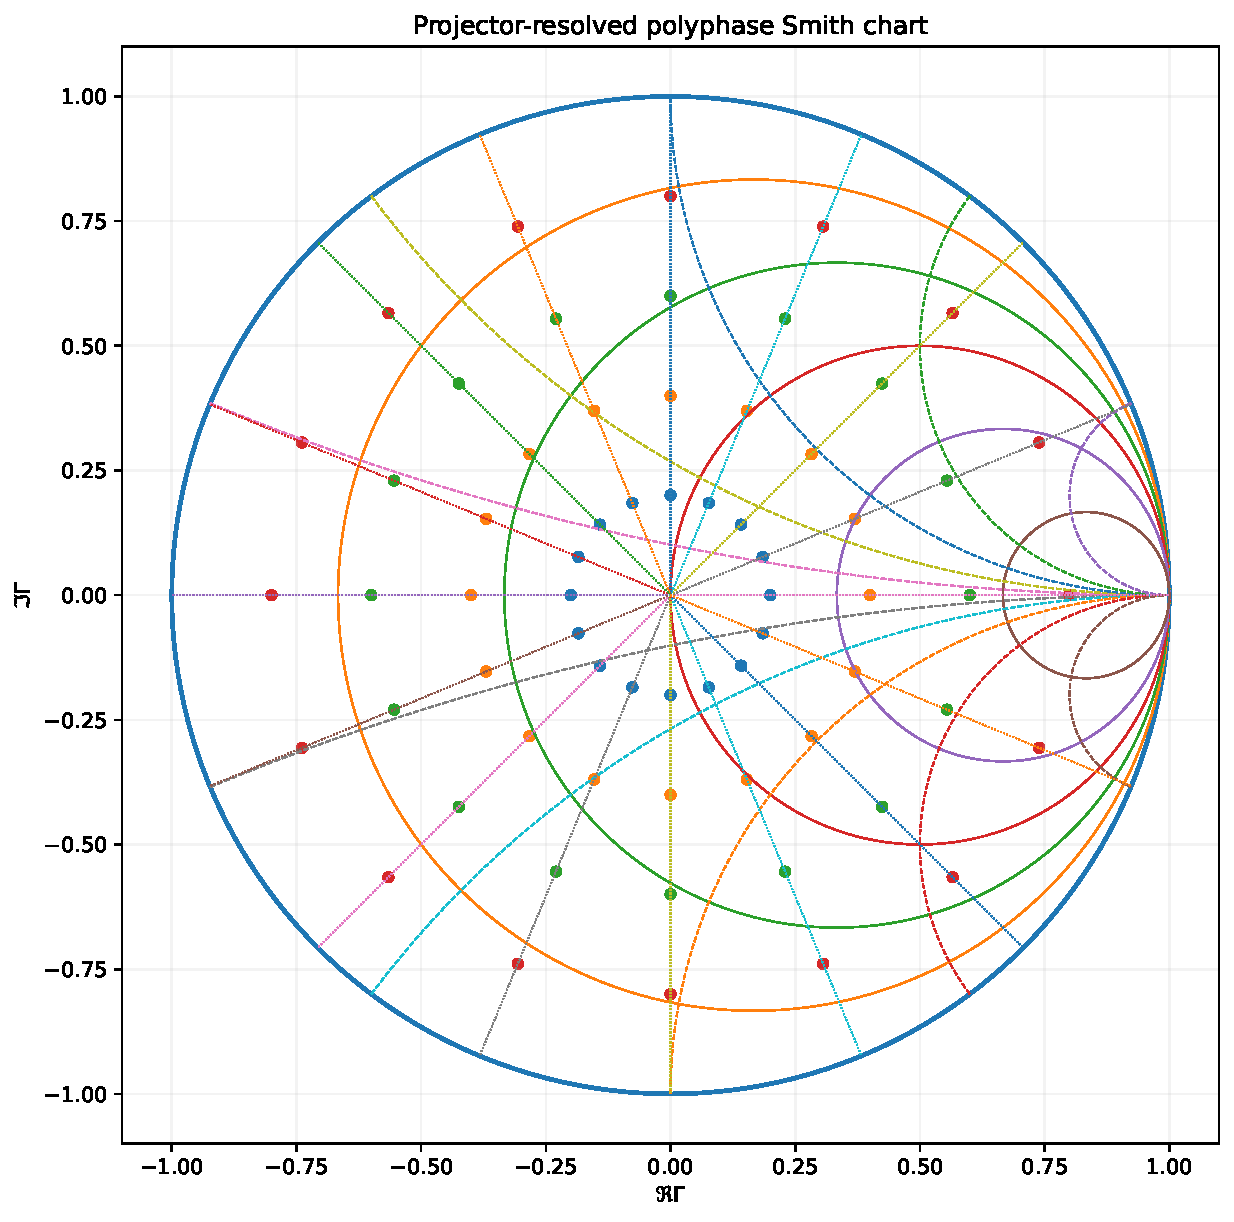
\includegraphics[width=0.88\textwidth]{11_polyphase_smith_chart.pdf}
\caption{The classical Smith grid equipped with sixteen exact phase rays and four radial seed orbits. The Cayley transform creates the chart; the projector calculus supplies the nested cyclic coordinate system.}
\label{fig:smith-chart}
\end{figure}

\subsection{Radial seeds and physical phase}

For $0\le\rho<1$ and angle $\theta$,
\[
\Gam=\rho e^{\ii\theta}
\]
gives
\[
z(\rho,\theta)
=\frac{1+\rho e^{\ii\theta}}{1-\rho e^{\ii\theta}},
\]
with
\[
r(\rho,\theta)=\frac{1-\rho^2}{1-2\rho\cos\theta+\rho^2},
\qquad
x(\rho,\theta)=\frac{2\rho\sin\theta}{1-2\rho\cos\theta+\rho^2}.
\]
A fixed $\rho$ is a constant-mismatch circle. Refining $N$ increases angular resolution without changing $\rho$.

\begin{figure}[htbp]
\centering
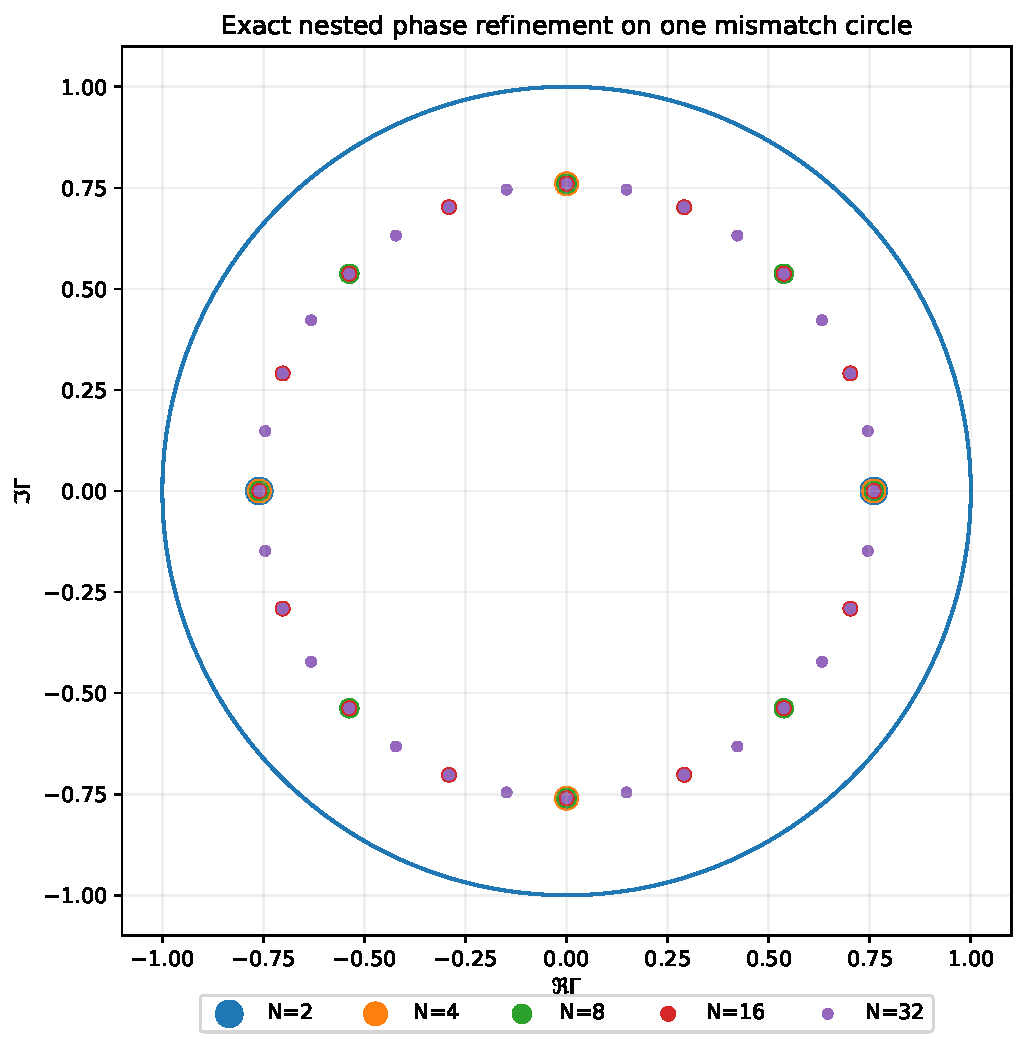
\includegraphics[width=0.78\textwidth]{12_smith_nested_refinement.pdf}
\caption{The same reflection circle at phase orders $2,4,8,16,32$. Coarse phase packets are exact unions of their fine descendants.}
\label{fig:smith-refinement}
\end{figure}

For a lossless transmission line,
\[
\Gam_{\rm in}=\Gam_L e^{-2\ii\beta\ell}.
\]
One $N$-phase step corresponds to a line-length increment $\lambda/(2N)$, up to the chosen orientation convention. Hence the phase address has a direct electrical interpretation.

\section{Dyadic--odd phase factorization and boundary weighting}

Write
\[
N=2^sM,
\qquad M\text{ odd}.
\]
The cyclic index splits by the Chinese remainder theorem:
\[
\bbZ/N\bbZ
\cong
\bbZ/2^s\bbZ\times\bbZ/M\bbZ.
\]

\begin{proposition}[Dyadic--odd packet factorization]
After identifying the residue labels by the Chinese remainder map, the phase projector factors as
\[
\boxed{
P_{N,j}=P_{2^s,j_2}P_{M,j_o}.
}
\]
\end{proposition}

\begin{proof}
The two congruence conditions are independent because $2^s$ and $M$ are coprime. Their indicator functions multiply to the indicator of the unique residue class modulo $N$ satisfying both.
\end{proof}

The first dyadic step is exceptional in Smith coordinates because it is the inversion $z\mapsto z^{-1}$. Higher dyadic levels refine the open/short duality into quarter-, eighth-, and finer phase sectors.

The inverse Cayley map has derivative
\[
\frac{dz}{d\Gam}=\frac{2}{(1-\Gam)^2},
\]
while normalized admittance has derivative proportional to $(1+\Gam)^{-2}$. This motivates the symmetric sensitivity
\[
\boxed{
w_{\rm Smith}(\Gam)
=
\frac1{|1-\Gam|^2}
+
\frac1{|1+\Gam|^2}.
}
\]

\begin{figure}[htbp]
\centering
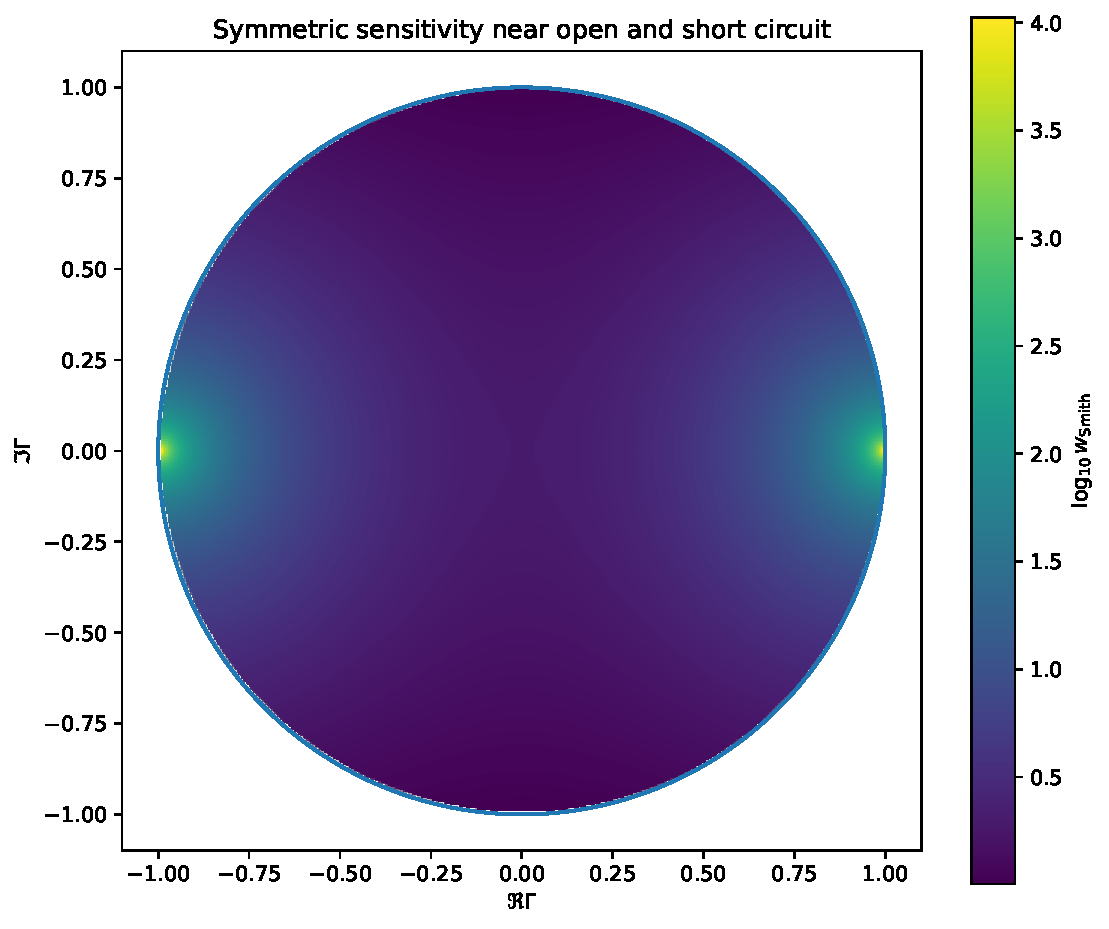
\includegraphics[width=0.78\textwidth]{13_smith_sensitivity.pdf}
\caption{The proposed symmetric refinement weight becomes large near the open- and short-circuit boundary points. It is a condition-based adaptive coordinate, not an asserted optimal sampling law.}
\label{fig:smith-weight}
\end{figure}

\begin{boundary}[Weighted refinement]
The sensitivity formula follows directly from the exact coordinate derivatives. Using it to choose an optimal adaptive grid, interpolation rule, or measurement design is a separate numerical problem. The release visualizes the weight but does not prove optimality.
\end{boundary}

\section{Boundary-localized error and claim control}

The strongest visual distinction between global Fourier reconstruction and exact packet retention is seen in a band around the discontinuity.

\begin{figure}[htbp]
\centering
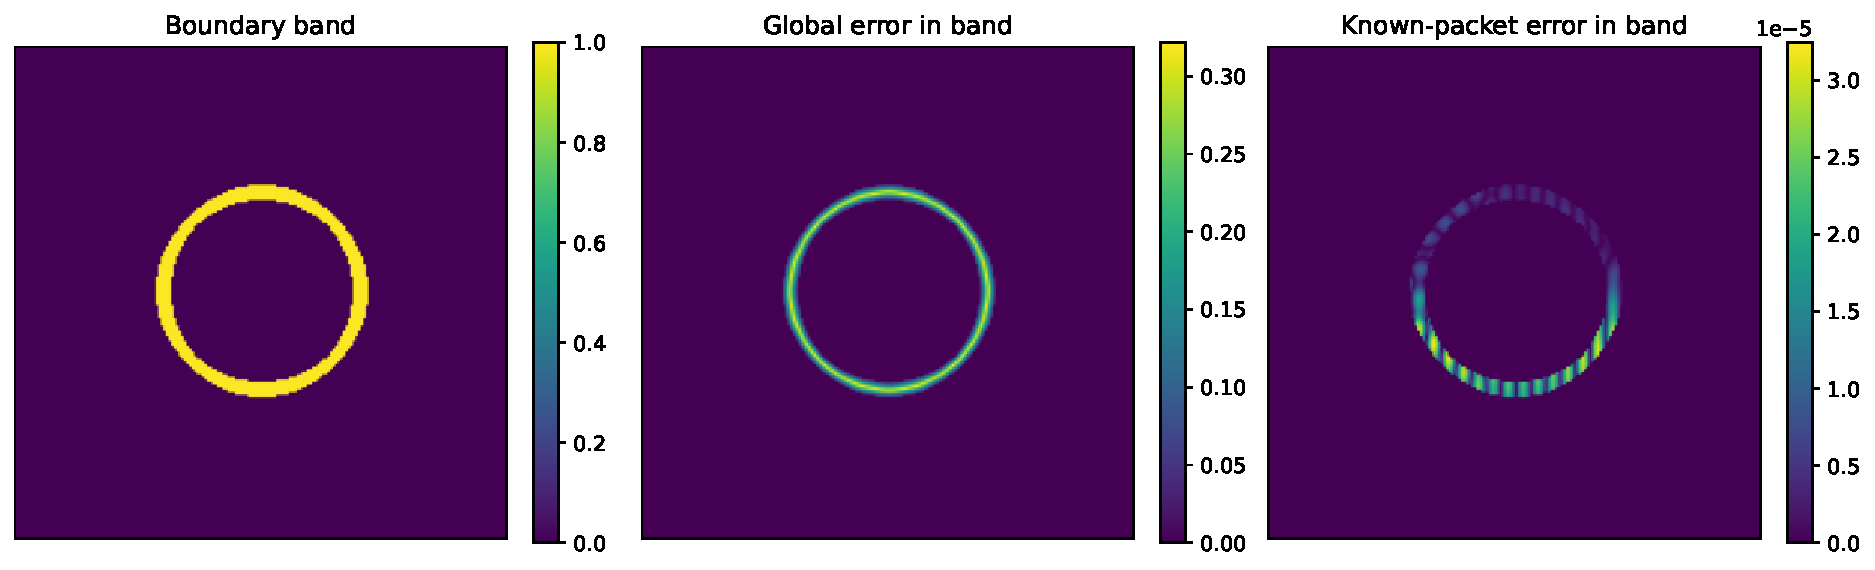
\includegraphics[width=0.94\textwidth]{15_boundary_leakage.pdf}
\caption{Error restricted to a narrow boundary band. Global truncation concentrates large error on the jump. The known-packet reconstruction has only the small smooth-packet error in the same band.}
\label{fig:boundary-error}
\end{figure}

\begin{figure}[htbp]
\centering
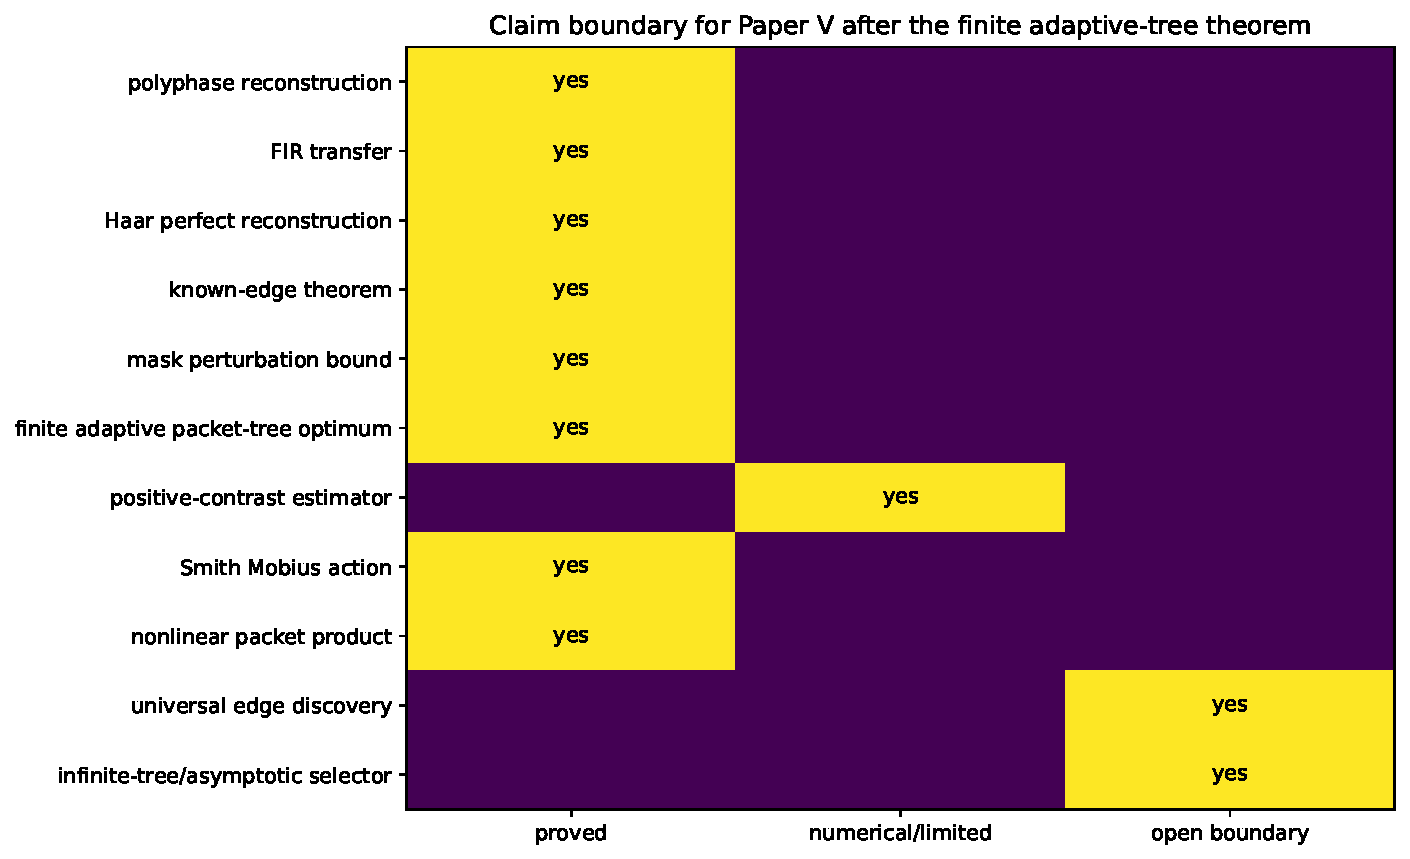
\includegraphics[width=0.90\textwidth]{16_claim_status.pdf}
\caption{Proof and claim boundary. Finite adaptive-tree selection is now proved; the remaining open rows concern universal recovery and infinite-tree or asymptotic selection.}
\label{fig:claim-status}
\end{figure}

\begin{conjecture}[Edge-packet approximation class]
There should exist natural function spaces in which a signal is represented as
\[
f=s+\sum_q a_q\mathbf1_{\Omega_q},
\]
with separate norms for smooth approximation, boundary geometry, packet amplitude, and packet identification. A projector-resolved approximation theory on such spaces should yield rates that do not mix smooth truncation error with discontinuity-location error.
\end{conjecture}


\section{Implementation and reproducibility}

The companion package is organized by mathematical layer:

\begin{longtable}{L{0.27\textwidth}L{0.64\textwidth}}
\toprule
\textbf{module}&\textbf{implemented content}\\
\midrule
\endfirsthead
\toprule
\textbf{module}&\textbf{implemented content}\\
\midrule
\endhead
\texttt{polyphase.py}&residue projectors, analysis/synthesis, refinement, exact FIR transfer kernels, polyphase convolution\\
\texttt{filterbanks.py}&Haar analysis/synthesis, complete Haar packet trees, energy accounting, predict--update lifting\\
\texttt{adaptive.py}&complete-pruning enumeration, exact mixed-depth synthesis, dynamic-programming optimization, and stability certificates\\
\texttt{edges.py}&one- and two-dimensional Fourier truncation, known-packet reconstruction, narrow two-class estimators, harmonic filling, error metrics\\
\texttt{smith.py}&Cayley coordinates, cyclic M\"obius action, Smith circles, sensitivity weight, coefficient projectors\\
\texttt{nonlinear.py}&coefficient packets, cyclic product convolution, nonlinear shifted packet reconstruction\\
\texttt{experiments.py}&all machine-readable numerical certificates and tabular summaries\\
\texttt{visuals.py}&the sixteen figure pairs used in the paper\\
\bottomrule
\end{longtable}

All computations in this paper are CPU-based. No GPU result is claimed. The exact theorems do not require numerical experiments; the computations verify the finite implementations and measure the specific synthetic examples.

\begin{certificate}[Exact finite residuals]
The largest recorded residuals were
\[
\begin{array}{lr}
\toprule
\text{identity}&\text{residual}\\
\midrule
\text{polyphase reconstruction}&0\\
\text{nested refinement}&0\\
\text{polyphase convolution}&4.44\times10^{-16}\\
\text{Haar reconstruction}&8.88\times10^{-16}\\
\text{wavelet-packet reconstruction}&2.22\times10^{-15}\\
\text{adaptive-tree optimum versus exhaustive search}&0\\
\text{adaptive mixed-depth synthesis}&8.88\times10^{-16}\\
\text{lifting reconstruction}&4.44\times10^{-16}\\
\text{Smith rotation conjugacy}&3.34\times10^{-16}\\
\text{Smith impedance--admittance duality}&0\\
\text{nonlinear product-packet reconstruction}&1.33\times10^{-15}\\
\text{nonlinear shifted-filter reconstruction}&0\\
\bottomrule
\end{array}
\]
The Haar and wavelet energy residuals were $5.68\times10^{-14}$ and $2.27\times10^{-13}$, respectively.
\end{certificate}

\section{Conclusions}

The signal realization gives one of the clearest demonstrations that the seed calculus is more than a verbal analogy. The objects and laws can be read directly:
\[
\boxed{
\begin{aligned}
\text{seed}&=\delta_0,\\
\text{address}&=S^n,\\
\text{packet}&=P_{N,r}x,\\
\text{transfer}&=P_{N,k}HP_{N,s},\\
\text{refinement}&=P_{N,r}=\sum_{s\succ r}P_{M,s},\\
\text{synthesis}&=\sum_rP_{N,r}x,\\
\text{nonlinearity}&=P_{N,r}F\left(\sum_sP_{N,s}x\right).
\end{aligned}
}
\]
Filter banks, wavelet packets, adaptive complete prunings, edge packets, and Smith coordinates inhabit the same operator grammar, but their claims differ. Polyphase and filter-bank identities are exact. Wavelet perfect reconstruction is exact. The known-edge theorem is exact conditional on the decomposition. Estimated-edge performance depends on a detection model. The Smith chart remains the classical Cayley geometry equipped with an exact cyclic refinement algebra. Keeping those distinctions explicit is part of the calculus, not an editorial afterthought.

The next paper in the series turns from discrete signal transfer to semigroups, resolvents, conditioning, stochastic evolution, fractional powers, and PDE kernels.

\appendix
\section{Algorithm statements}

\subsection{Exact polyphase filtering}

Given $x$, $h$, and $N$:

\begin{enumerate}
\item Form $x_s[n]=x[Nn+s]$ for $0\le s<N$.
\item Form every transfer kernel $h_{ks}[m]=h[Nm+k-s]$.
\item Compute
\[
y_k[n]=\sum_s\sum_mh_{ks}[m]x_s[n-m].
\]
\item Interleave the $y_k$ channels.
\end{enumerate}

The algorithm is algebraically identical to direct convolution; its purpose is to expose independent and interacting packets for block computation and refinement.

\subsection{Conditional known-edge reconstruction}

Given a decomposition $f=s+j$:

\begin{enumerate}
\item Apply the selected smooth approximation $Q_m$ to $s$ only.
\item Retain $j$ exactly.
\item Return $Q_ms+j$.
\end{enumerate}

The error certificate is $\|s-Q_ms\|$.

\subsection{Limited positive-contrast estimator}

The included finite estimator does the following:

\begin{enumerate}
\item Split the observed values into two classes by an Otsu threshold.
\item Keep coherent connected components and fill holes.
\item Harmically fill the selected packet to estimate the missing background.
\item Smooth the filled background spectrally.
\item Estimate one packet amplitude by a robust median residual.
\item Recombine the estimated smooth and edge packets.
\end{enumerate}

This procedure is useful for the supplied separated synthetic case. It assumes a positive-contrast two-class packet and is not promoted to a general edge theorem.

\section{Numerical record}

\begin{table}[H]
\centering
\caption{Main edge-study measurements.}
\begin{tabular}{lrrr}
\toprule
\text{case}&\text{global RMSE}&\text{known-packet RMSE}&\text{estimated RMSE}\\
\midrule
1D rectangular packet&$5.4023\times10^{-2}$&$1.3692\times10^{-4}$&$2.4029\times10^{-2}$\\
2D disk packet&$3.7643\times10^{-2}$&$6.4752\times10^{-5}$&$3.4043\times10^{-3}$\\
2D multiedge packet&$3.3740\times10^{-2}$&\multicolumn{2}{c}{known composite packet only}\\
\bottomrule
\end{tabular}
\end{table}

\begin{table}[H]
\centering
\caption{Main software artifacts.}
\begin{tabular}{ll}
\toprule
\text{artifact}&\text{purpose}\\
\midrule
\texttt{results/numerical\_results.json}&complete machine-readable certificate record\\
\texttt{tables/numerical\_summary.csv}&flat summary of errors and residuals\\
\texttt{tables/sparse\_representation.csv}&wavelet/Fourier coefficient study\\
\texttt{tests/}&automated finite identity and estimator tests\\
\texttt{figures/}&PNG and vector-PDF figure pairs\\
\texttt{Run\_All.ps1}&Windows generation, testing, wheel, and PDF runner\\
\bottomrule
\end{tabular}
\end{table}

\section{Notation crosswalk}

\begin{longtable}{L{0.20\textwidth}L{0.33\textwidth}L{0.37\textwidth}}
\toprule
\textbf{common symbol}&\textbf{signal realization}&\textbf{interpretation}\\
\midrule
\endfirsthead
\toprule
\textbf{common symbol}&\textbf{signal realization}&\textbf{interpretation}\\
\midrule
\endhead
$s$&$\delta_0$&primitive signal seed\\
$A_n$&$S^n$&address operator\\
$P_{N,r}$&residue mask&phase packet projector\\
$T_{ks}$&$P_{N,k}HP_{N,s}$&input-to-output phase transfer\\
$E,R$&analysis and synthesis matrices&coordinate conversion and reconstruction\\
$W(\gamma)$&filter or path weight&refinement or implementation cost\\
$\Delta(F)$&coarse/fine signal defect&aliasing, leakage, or estimator inconsistency\\
$\operatorname{Hol}(\gamma)$&closed phase transfer&cycle consistency in a network\\
$\Gam$&reflection coefficient&Smith-disk coordinate\\
\bottomrule
\end{longtable}

\end{document}
